\documentclass[aspectratio=1610,mathserif]{beamer}

%\usetheme{Madrid}
\usecolortheme{orchid}

\usepackage{amsmath}
\usepackage{amssymb}
\usepackage{graphicx}
\usepackage{hyperref}
\usepackage{minted}
\usepackage{stmaryrd}
\usepackage{ebproof}
\usepackage{tikz-cd}
\usepackage{subcaption}
\usepackage[table]{xcolor}
\usepackage{booktabs}

\definecolor[named]{ACMBlue}{cmyk}{1,0.1,0,0.1}
\definecolor[named]{ACMYellow}{cmyk}{0,0.16,1,0}
\definecolor[named]{ACMOrange}{cmyk}{0,0.42,1,0.01}
\definecolor[named]{ACMRed}{cmyk}{0,0.90,0.86,0}
\definecolor[named]{ACMLightBlue}{cmyk}{0.49,0.01,0,0}
\definecolor[named]{ACMGreen}{cmyk}{0.20,0,1,0.19}
\definecolor[named]{ACMPurple}{cmyk}{0.55,1,0,0.15}
\definecolor[named]{ACMDarkBlue}{cmyk}{1,0.58,0,0.21}

\usetikzlibrary{arrows.meta,positioning,fit,calc,overlay-beamer-styles}

% helpers: keep layout but hide visually
\tikzset{
  invisible/.style={opacity=0,text opacity=0},
  visible on/.style={alt={#1{}{invisible}}},
}

% node helper that reserves space when hidden
\newcommand<>{\showon}[1]{\alt#2{#1}{\phantom{#1}}}

\AtBeginSection{
  \frame{\sectionpage}
}

\newcommand{\todo}[1]{\textcolor{red}{#1}}
\newcommand{\kw}[1]{\ensuremath{ \mathsf{#1} }}
\newcommand{\C}{\ensuremath{ \mathcal{C} }}
\newcommand{\A}{\ensuremath{ \mathcal{A} }}
\newcommand{\que}{\circ}         % superscript for questions
\newcommand{\ans}{\bullet}       % superscript for answers
\newcommand{\termi}[1]{\langle {#1} ]}
\newcommand{\encap}[1]{[ {#1} \rangle}
\newcommand{\at}{\mathbin@}
\newcommand{\red}[1]{\textcolor{red}{#1}}
\newcommand{\ifr}[1]{\mathrel{[{#1}]}}
\newcommand{\idsc}{\mathbf{id}} % identity simulation convention
\newcommand{\intl}[1]{#1^0}
\newcommand{\envstep}{\leadsto}
\newcommand{\sysstep}{\rightarrowtail}
\newcommand{\emptysig}{0}
\newcommand{\vcomp}{\fatsemi}
\newcommand{\jr}{\mathsf{Y}}
\newcommand*{\twoheadleftrightarrow}{%
  \twoheadleftarrow
  \mathrel{\mkern-15mu}%
  \twoheadrightarrow
}
\newcommand{\lensarrow}{\rightleftarrows}

\title{Building Certified Systems with Compositional Semantics}
\author{Yu Zhang}
\institute{Yale University}
\date{\today}

\begin{document}

\begin{frame}
  \titlepage
\end{frame}

\begin{frame}{Outline}
  \tableofcontents
\end{frame}

\section{Introduction}

\begin{frame}{Common Verification Tasks}
  Much real-world programming follows two recurring patterns:
  \begin{itemize}
    \item Library code implementing specific data structures or algorithms
    \item Executables that are algorithmically simple but interact extensively with their external environment
  \end{itemize}
\end{frame}

\begin{frame}[fragile]{Bounded Queue Example}
  \captionof{listing}{Compilation unit $\kw{rb.c}$ implementing a ring buffer}
  \vspace{-0.8em}
  \begin{minted}[fontsize=\footnotesize,frame=single,numbersep=0.3em]{c}
static int c1, c2;
static V buf[N];

int inc1() { int i = c1++; c1 %= N; return i; }
int inc2() { int i = c2++; c2 %= N; return i; }
V get(int i) { return buf[i]; }
void set(int i, V val) { buf[i] = val; }
  \end{minted}
  \vspace{0.5em}
  \captionof{listing}{Compilation unit $\kw{bq.c}$ implementing a bounded queue}
  \vspace{-0.8em}
  \begin{minted}[fontsize=\footnotesize,frame=single,numbersep=0.3em]{c}
extern int inc1(void);
extern int inc2(void);
extern V get(int i);
extern void set(int i, V val);

void enq(V val) { set(inc2(), val); }
V deq() { return get(inc1()); }
  \end{minted}
\end{frame}

\begin{frame}[fragile]{Rot13 Example}
  \begin{columns}
  \begin{column}{0.41\textwidth}
    \captionof{listing}{$\kw{secret.s}$}
    \vspace{-0.8em}
    \begin{minted}[fontsize=\footnotesize,frame=single,numbersep=0.3em]{gas}
.globl main
main:   pushl $13
      pushl $msg
      call rot13
      pushl $1
      call write
      addl $12, %esp
      movl $0, %eax
      ret
.data
msg:    .string "hello, world!\n"
    \end{minted}
    \begin{minted}[fontsize=\footnotesize,frame=single,numbersep=0.3em]{bash}
$ cc -o secret secret.s rot13.c
$ ./secret
uryyb, jbeyq!
$ cc -o decode decode.c rot13.c
$ ./secret | ./decode
hello, world!
    \end{minted}
  \end{column}
  \begin{column}{0.595\textwidth}
    \captionof{listing}{$\kw{rot13.c}$}
    \vspace{-0.8em}
    \begin{minted}[fontsize=\footnotesize,frame=single,numbersep=0.3em]{c}
void rot13(char *buf, int len) {
  for (int i = 0; i < len; i++)
    if ('a' <= buf[i] && buf[i] <= 'z')
      buf[i] = (buf[i] - 'a' + 13) % 26 + 'a';
}
    \end{minted}
    \vspace{1em}
    \captionof{listing}{$\kw{decode.c}$}
    \vspace{-0.8em}
    \begin{minted}[fontsize=\footnotesize,frame=single,numbersep=0.3em]{c}
#include <unistd.h>
extern void rot13(char *, int);
int main() {
  char buf[100];
  int n = read(0, buf, sizeof buf);
  rot13(buf, n);
  write(1, buf, n);
  return 0;
}
    \end{minted}
  \end{column}
\end{columns}

\end{frame}

\begin{frame}{Problem Statement}
  To enable the verification of large-scale software systems,
  the framework must account for the following aspects:
  \begin{enumerate}
    \item Supporting multiple levels of abstraction
    \item Reasoning in open context
    \item State encapsulation
    \item Compilation correctness, linking and loading
    \item Multi-language components
  \end{enumerate}
\end{frame}

\begin{frame}[fragile]{Challenge 1: Supporting Multiple Levels of Abstraction}

  Considered the example of a bounded queue.
  There are multiple perspectives to describe the system.
  \begin{columns}
    \begin{column}{0.75\textwidth}
      \begin{itemize}
        \item<1-> First-in, first-out property
          \[
            \kw{enq}(v_1) \prec \kw{enq}(v_2) \quad \Longrightarrow \quad \kw{deq}(v_1) \prec \kw{deq}(v_2)
          \]
        \item<2-> Functional program
          \begin{columns}
            \begin{column}{0.45\textwidth}
    \begin{minted}[fontsize=\footnotesize,frame=single]{haskell}
enq :: a -> [a] -> [a]
enq v q = q ++ [v]
    \end{minted}
            \end{column}
            \begin{column}{0.45\textwidth}
    \begin{minted}[fontsize=\footnotesize,frame=single]{haskell}
deq :: [a] -> (a, [a])
deq (v : q) = (v, q)
    \end{minted}
            \end{column}
          \end{columns}
          \vspace{1em}
        \item<3-> C programs: $\kw{bq.c}$ and $\kw{rb.c}$
      \end{itemize}
    \end{column}
    \begin{column}{0.25\textwidth}
      \[
        \vspace{-3em}
        \begin{array}{c}
          \text{$\kw{Spec}_\kw{relational}$}\\[1em]
          \only<2->{\raisebox{0.5em}{\rotatebox{270}{$\sqsubseteq$}}}\\[1em]
          \only<2->{\text{$\kw{Spec}_\kw{functional}$}}\\[1em]
          \only<3->{\raisebox{0.5em}{\rotatebox{270}{$\sqsubseteq$}}}\\[1em]
          \only<3->{\text{$\kw{bq.c} + \kw{rb.c}$}}\\[1em]
        \end{array}
      \]
    \end{column}
  \end{columns}
\end{frame}

\begin{frame}[fragile]{Challenge 1: Supporting Multiple Levels of Abstraction}
  Data abstraction is an important aspect
  of supporting multiple levels of abstraction.
  \begin{itemize}
    \item Sequence of values
      \[
        \kw{nil} \xrightarrow{\kw{enq}(v_1)}\ [v_1]
        \ \xrightarrow{\kw{enq}(v_2)}\ [v_1, v_2]
        \ \xrightarrow{\ \ \kw{deq}\ \ }\ v_1, [v_2]
      \]
      \pause
    \item Fixed-size buffer with two counters
      \begin{align*}
        ([\kw{undef}, \kw{undef}, \cdots], 0, 0)
        \ \xrightarrow{\kw{enq}(v_1)}\ &
        ([v_1, \kw{undef}, \cdots], 1, 0)\\
        \ \xrightarrow{\kw{enq}(v_2)}\ &
        ([v_1, v_2, \cdots], 2, 0)\\
        \ \xrightarrow{\ \ \kw{deq}\ \ }\ &
        v_1, ([v_1, v_2, \cdots], 2, 1)
      \end{align*}
      \pause
    \item Memory representation
  \end{itemize}
\end{frame}

\begin{frame}[fragile]{Closed-Universe Assumption}
  \begin{minted}[fontsize=\footnotesize,frame=single,numbersep=0.3em]{c}
void enq(V val) { set(inc2(), val); }
V deq() { return get(inc1()); }
  \end{minted}

  In closed-semantics,
  the behavior of $\kw{bq.c}$ is unclear
  without having the behavior of the underlying ring buffer functions provided in advance.
  \pause
  \vspace{1em}
  \begin{itemize}
    \item Option 1: Verify $\kw{bq.c}$ together with $\kw{rb.c}$
      \begin{itemize}
        \item Not modular
      \end{itemize}
      \pause
    \item Option 2: Use $\kw{Spec}_\kw{rb}$ as the behavior of $\kw{rb.c}$.
      \begin{itemize}
        \item Must verify $\kw{rb.c}$ against $\kw{Spec}_\kw{rb}$ first
        \item The semantics and data representation of $\kw{Spec}_\kw{rb}$
          must be fixed in this scenario.
      \end{itemize}
  \end{itemize}
\end{frame}

\begin{frame}[fragile]{Challenge 2: Reasoning in Open Context}
  \begin{minted}[fontsize=\footnotesize,frame=single,numbersep=0.3em]{c}
void enq(V val) { set(inc2(), val); }
V deq() { return get(inc1()); }
  \end{minted}

  Open-world reasoning: verify components in isolation.
  \pause
  \\[0.5ex]
  \begin{itemize}
    \item For example, the specification of $\kw{bq.c}$ can be expressed as:
      \begin{itemize}
        \item If it is called via $\kw{enq}(v_1)$,
        \item it will call $\kw{inc_2}()$,
        \item and if integer $i$ is returned, it will call $\kw{set}(i, v_1)$
      \end{itemize}
      \pause
    \item Only the \textbf{interaction interface} of the ring buffer is fixed.
      \pause
    \item This specification can also be expressed as the following trace of events:
      \[
        \kw{Spec}_\kw{bq} \ \vDash\ \kw{enq}(v_1)
        \ \cdot\ \underline{\kw{inc_2}()}
        \ \cdot\ i
        \ \cdot\ \underline{\kw{set}(i, v_1)}
        \ \cdot\ *
        \ \cdot\ \underline{*}
      \]
  \end{itemize}
\end{frame}

\begin{frame}[fragile]{Challenge 2: Reasoning in Open Context---Example with Processes}
  \begin{itemize}
    \item Reasoning about two processes communicating via pipes.
  \end{itemize}
  \begin{minted}[fontsize=\footnotesize,frame=single,numbersep=0.3em]{bash}
$ ./secret | ./decode
hello, world!
  \end{minted}

  \begin{itemize}
    \item One process cannot hard-code the other's behavior.
    \item $\kw{decode}$ must handle all possible inputs from $\kw{secret}$.
  \end{itemize}
  \vspace{1em}
  \pause
  More generally, open context arises in the following scenarios:
  \begin{itemize}
    \item Device drivers with arbitrary hardware signals
    \item OS kernel interacting with unverified or foreign modules
    \item Services that are not started by calling the main function
  \end{itemize}
\end{frame}

\begin{frame}{Challenge 3: State Encapsulation}
  \begin{itemize}
    \item Low level state: all components share a global memory state
    \item High level state: partition and encapsulate the abstract state
  \end{itemize}
  \pause
  \vspace{1em}
  From the view of the client of the bounded queue:
  \begin{itemize}
    \item Explicit state-passing
      \[
        \kw{enq}(v_1) \at \kw{nil} \ \cdot\
        \underline{* \at [v_1]} \ \cdot\
        \kw{enq}(v_2) \at [v_1] \ \cdot\
        \underline{* \at [v_1, v_2]} \ \cdot\
        \kw{deq} \at [v_1, v_2] \ \cdot\
        \underline{v_1 \at [v_2]}
      \]
    \item State encapsulation
      \[
        \kw{enq}(v_1) \ \cdot\
        \underline{*} \ \cdot\
        \kw{enq}(v_2) \ \cdot\
        \underline{*} \ \cdot\
        \kw{deq} \ \cdot\
        \underline{v_1}
      \]
  \end{itemize}
\end{frame}

\begin{frame}{Challenge 4: Compile, Link, and Load}
  To achieve end-to-end verification,
  we must prove correctness across three stages:
  compilation, linking, and loading.
  {\small
    \[
      \begin{array}{cl}
        \only<1->{\text{$\kw{Spec}_\kw{decode}$}}&
        \only<1->{\text{(overall specification)}}
        \\[0.5em]
        \only<1->{\raisebox{0.5em}{\rotatebox{270}{$\sqsubseteq$}}}&
        \only<1->{\text{(manual proof)}}
        \\[0.5em]
        \only<1->{\text{$\kw{Spec}_\kw{decode.c} \oplus \kw{Spec}_\kw{rot13.c}$}}&
        \only<1->{\text{(program-level specification)}}
        \\[0.5em]
        \only<2->{\raisebox{0.5em}{\rotatebox{270}{$\sqsubseteq$}}}&
        \only<2->{\text{(manual proof)}}
        \\[0.5em]
        \only<2->{\text{$\llbracket \kw{decode.c} \rrbracket \oplus \llbracket \kw{rot13.c} \rrbracket$}}&
        \only<2->{\text{(composite C-level components)}}
        \\[0.5em]
        \only<3->{\raisebox{0.5em}{\rotatebox{270}{$\sqsubseteq$}}}&
        \only<3->{\text{\textbf{compiler correctness}}}
        \\[0.5em]
        \only<3->{\text{$\llbracket \kw{decode.s} \rrbracket \oplus \llbracket \kw{rot13.s} \rrbracket$}}&
        \only<3->{\text{(composite assembly-level components)}}
        \\[0.5em]
        \only<4->{\raisebox{0.5em}{\rotatebox{270}{$\sqsubseteq$}}}&
        \only<4->{\text{\textbf{linking correctness}}}
        \\[0.5em]
        \only<4->{\text{$\llbracket \kw{decode.s} + \kw{rot13.s} \rrbracket$}}&
        \only<4->{\text{(linked assembly program)}}
        \\[0.5em]
        \only<5->{\raisebox{0.5em}{\rotatebox{270}{$\sqsubseteq$}}}&
        \only<5->{\text{\textbf{loading into execution environment}}}\\[0.5em]
        \only<5->{\text{$\kw{load}(\llbracket \kw{decode.s} + \kw{rot13.s} \rrbracket)$}}&
      \end{array}
    \]
  }
\end{frame}

\begin{frame}{Challenge 5: Heterogeneous Components}
  It is common that a software system is written using different programming languages.
  \begin{itemize}
    \item Hand-written assembly code for better performance
    \item Functionality cannot be written in high-level languages when writing OS kernel
      \pause
    \item $\kw{secret.s}$ in the rot13 example as a concrete example
  \end{itemize}
  \begin{minted}[fontsize=\footnotesize,frame=single,numbersep=0.3em]{bash}
$ cc -o secret secret.s rot13.c
$ ./secret
uryyb, jbeyq!
\end{minted}

  \pause
  \begin{itemize}
    \item The pipe itself is a heterogeneous component.
  \end{itemize}
  The verification framework must incorporate the heterogeneity
  seamlessly in a unified model.
\end{frame}

\begin{frame}{Existing Approaches are Insufficient}
  \textbf{Semantic model} is the key to verification.
  \begin{itemize}
    \item<1-> Operational semantics and program logic
      \begin{itemize}
        \item Fixed semantic model and interaction patterns
        \item New models are required for new tasks
      \end{itemize}
    \item<2-> Denotational semantics
      \begin{itemize}
        \item Not connect with practical compiler correctness
        \item Gap between semantic models and notion of correctness
      \end{itemize}
    \item<3-> Compositional certified compiler (a.k.a. open semantics)
      \begin{itemize}
        \item Focus on compiler correctness
        \item Lack of state abstraction and encapsulation
      \end{itemize}
    \item<4-> Game semantics
      \begin{itemize}
        \item Lack of support for different abstraction levels
      \end{itemize}
  \end{itemize}

\end{frame}

\begin{frame}{My Contributions}
  This work develops a generic verification framework built with:
  \begin{itemize}
    \item Strategy model
    \item Refinement conventions and refinement squares
    \item \textbf{Three-dimensional algebraic composition structure}
  \end{itemize}
  \vspace{1em}
  \pause
  The framework is capable of:
  \begin{itemize}
    \item Verifying examples from the introduction
    \item Incorporating CompCertO's semantics and compiler correctness
    \item Implementing Certified Abstraction Layers (CAL)
  \end{itemize}
  \pause
  The framework is mechanized in Rocq.

\end{frame}

\section{Overview of the Framework}

\begin{frame}{Overview of the Strategy Model}
  Core ingredients:
  \begin{itemize}
    \item Effect signature: \textbf{question} events
      and \textbf{answer} events
      \[
        E_\kw{bq} := \{ \kw{enq}[v], \only<2->{*,} \kw{deq}, \only<2->{v,} \cdots \}\qquad \qquad
        E_\kw{rb} := \{ \kw{inc_1}, \kw{inc_2}, \only<2->{i,} \kw{get}[i], \only<2->{v,} \kw{set}(i, v), \only<2->{*,} \cdots \}
      \]
      \pause
      \pause
    \item Strategy describes component behaviors
      \begin{columns}
        \begin{column}{.3\textwidth}
          \[
            \sigma_\kw{bq} : E_\kw{rb} \rightarrow E_\kw{bq}
          \]
        \end{column}
        \begin{column}{.5\textwidth}
          \[
            \hspace{-6em}
            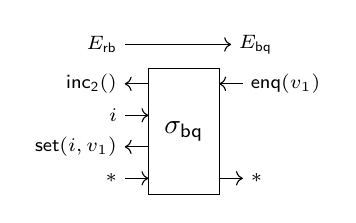
\begin{tikzpicture}[yscale=0.2,xscale=0.3]
              \draw (1,-1) rectangle (4,7) node[midway] {$\sigma_\kw{bq}$};
              \scriptsize
              \draw[<-] (0,6) node[left] {$\kw{inc_2}()$} -- (1,6);
              \draw[<-] (4,6) -- (5,6) node[right] {$\kw{enq}(v_1)$};
              \draw[->] (0,4) node[left] {$i$} -- (1,4) ;
              \draw[<-] (0,2) node[left] {$\kw{set}(i, v_1)$} -- (1,2);
              \draw[<-] (5,0) node[right] {$*$} -- (4,0);
              \draw[<-] (1,0) -- (0,0) node[left] {$*$};
              \draw[->] (0,8.5) node[left] {$E_\kw{rb}$} -- (4.5,8.5) node[right] {$E_\kw{bq}$};
            \end{tikzpicture}
          \]
        \end{column}
      \end{columns}
      \pause
    \item Strategy composition
      \begin{columns}
        \begin{column}{.3\textwidth}
          \[
            \mathbf{0}
            \xrightarrow{\sigma_\kw{rb}} E_\kw{rb}
            \xrightarrow{\sigma_\kw{bq}} E_\kw{bq}
          \]
        \end{column}
        \begin{column}{.5\textwidth}
          \[
            \hspace{-5em}
            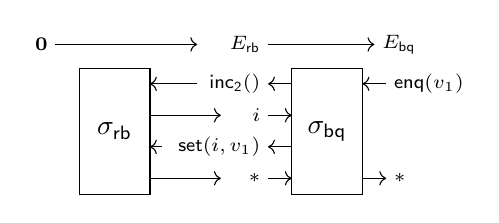
\begin{tikzpicture}[yscale=0.2,xscale=0.3]
              \draw (-8,-1) rectangle (-5,7) node[midway] {$\sigma_\kw{rb}$};
              \draw (1,-1) rectangle (4,7) node[midway] {$\sigma_\kw{bq}$};
              \scriptsize
              % bq arrows
              \draw[<-] (0,6) node[left] {$\kw{inc_2}()$} -- (1,6);
              \draw[<-] (4,6) -- (5,6) node[right] {$\kw{enq}(v_1)$};
              \draw[->] (0,4) node[left] {$i$} -- (1,4) ;
              \draw[<-] (0,2) node[left] {$\kw{set}(i, v_1)$} -- (1,2);
              \draw[<-] (5,0) node[right] {$*$} -- (4,0);
              \draw[<-] (1,0) -- (0,0) node[left] {$*$};
              \draw[->] (0,8.5) node[left] {$E_\kw{rb}$} -- (4.5,8.5) node[right] {$E_\kw{bq}$};
              % rb arrows
              \draw[<-] (-5,6) -- (-3,6);
              \draw[->] (-5,4) -- (-2,4);
              \draw[<-] (-5,2) -- (-4.5,2);
              \draw[->] (-5,0) -- (-2,0);
              \draw[->] (-9,8.5) node[left] {$\mathbf{0}$} -- (-3,8.5);
            \end{tikzpicture}
          \]
        \end{column}
      \end{columns}
  \end{itemize}
\end{frame}

\begin{frame}{Effect Signature}
  The semantic model uses \textbf{effect signature}
  as the interaction interfaces.

  \begin{definition}[Effect signature]
    A set $E$ of questions, and for each $m \in E$ a set of answers $N$.
    Written $\{ m : N \}$.
  \end{definition}
  \pause
  \begin{example}[Effect signature]
    The following signatures are used:
    \begin{align*}
      \visible<2->{E_\kw{rb} & := \{ \kw{inc_1} : \mathbb{N},\ \kw{inc_2} : \mathbb{N},\
          \kw{get}[i] : V,\ \kw{set}(i, v) : \{ * \} \mid
        i \in \mathbb{N}, v \in V \} \\
      E_\kw{bq} & := \{ \kw{enq}[v] : \{ * \},\ \kw{deq}:V \mid v \in V \}}\\
      \visible<3->{\mathcal{C} \at \kw{mem} & :=
        \{ f(\vec{v}) \at m : \kw{val} \times \kw{mem} \mid
        f \in \kw{val}, \vec{v} \in \kw{val}^*, m \in \kw{mem} \}\\
        \mathcal{A} \at \kw{mem} & :=
        \{ rs \at m : \kw{val}^* \times \kw{mem} \mid
      rs \in \kw{val}^*, m \in \kw{mem} \}} \\
      \visible<4->{\mathcal{P} & := \{ \kw{run} : \mathbb{N} \}\\
        \mathcal{S} & := \{ \kw{read}_i[n] : \kw{bytes},\ \kw{write}_i[s] : \mathbb{N}
      \mid i \in \mathbb{N}, n \in \mathbb{N}, s \in \kw{bytes}  \}}
    \end{align*}
  \end{example}
\end{frame}

\begin{frame}{Strategies}
  Models component behavior as \textbf{interaction events}
  \begin{itemize}
    \item $\sigma : E \rightarrow F$ specifies a component \emph{using} $E$ to \emph{implement} $F$
      \pause
    \item Naturally models open context
      \begin{columns}[t]
        \begin{column}[t]{.6\textwidth}
          \vspace{-2ex}
          \[
            \sigma_\kw{bq} : E_\kw{rb} \rightarrow E_\kw{bq} \ \vDash\ \kw{enq}(v_1)
            \ \cdot\ \underline{\kw{inc_2}()}
            \ \cdot\ i
            \ \cdot\ \underline{\kw{set}(i, v_1)}
            \ \cdot\ *
            \ \cdot\ \underline{*}
          \]
        \end{column}
        \begin{column}[t]{.4\textwidth}
          \vspace{-2ex}
          \[
            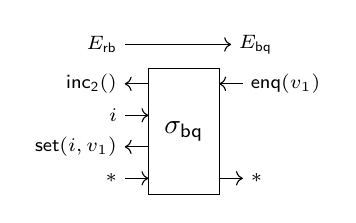
\begin{tikzpicture}[yscale=0.2,xscale=0.3]
              \draw (1,-1) rectangle (4,7) node[midway] {$\sigma_\kw{bq}$};
              \scriptsize
              \draw[<-] (0,6) node[left] {$\kw{inc_2}()$} -- (1,6);
              \draw[<-] (4,6) -- (5,6) node[right] {$\kw{enq}(v_1)$};
              \draw[->] (0,4) node[left] {$i$} -- (1,4) ;
              \draw[<-] (0,2) node[left] {$\kw{set}(i, v_1)$} -- (1,2);
              \draw[<-] (5,0) node[right] {$*$} -- (4,0);
              \draw[<-] (1,0) -- (0,0) node[left] {$*$};
              \draw[->] (0,8.5) node[left] {$E_\kw{rb}$} -- (4.5,8.5) node[right] {$E_\kw{bq}$};
            \end{tikzpicture}
          \]
        \end{column}
      \end{columns}
      \vspace{-1.5ex}
      \pause
    \item State as interaction history
      \[
        \sigma_\kw{queue} \ \vDash\
        \kw{enq}(v_1)
        \ \cdot\ \underline{*}
        \ \cdot\ \kw{enq}(v_2)
        \ \cdot\ \underline{*}
        \ \cdot\ \kw{deq}
        \ \cdot\ \underline{v_1}
        \ \cdots
      \]
  \end{itemize}
\end{frame}

\begin{frame}{Strategies---Program Semantics}
  \begin{itemize}
    \item CompCertO program semantics
      \[
        \kw{Clight}(p.c) : \mathcal{C} \at \kw{mem} \rightarrow \mathcal{C} \at \kw{mem}
        \qquad \qquad
        \kw{Asm}(p.s) : \mathcal{A} \at \kw{mem} \rightarrow \mathcal{A} \at \kw{mem}
      \]
  \end{itemize}
  \pause
  \begin{block}{Example}
    The strategies for the program $\kw{decode.c}$ exhibit traces such as:
    \begin{align*}
      \kw{Clight}(\kw{decode.c}) \:\vDash\:
      & \kw{main}()@m\ \cdot \\
      & \underline{\kw{read}(0, b, 100)@m[b \mapsto \textit{unspecified}]} \ \cdot \\
      & 14@m[b \mapsto \texttt{"uryyb, jbeyq!\textbackslash{}n"}] \ \cdot \\
      & \underline{\kw{rot13}(b, 14)@m[b \mapsto \texttt{"uryyb, jbeyq!\textbackslash{}n"}]} \ \cdot \\
      & {*}@m[b \mapsto \texttt{"hello, world!\textbackslash{}n"}] \ \cdot \\
      & \underline{\kw{write}(1, b, 14)@m[b \mapsto \texttt{"hello, world!\textbackslash{}n"}]} \ \cdot \\
      & 14@m[b \mapsto \texttt{"hello, world!\textbackslash{}n"}] \ \cdot \\
      & \underline{0@m[b \mapsto \textit{deallocated}]}
    \end{align*}
  \end{block}
\end{frame}

\begin{frame}{Strategies---Process Semantics}
  \begin{itemize}
    \item Process semantics
      \[
        \Gamma_\kw{decode} : \mathcal{S} \rightarrow \mathcal{P}
        \qquad \qquad
        \kw{load}(\kw{Asm}(p.s)) : \mathcal{S} \rightarrow \mathcal{P}
      \]
  \end{itemize}
  \pause
  \begin{block}{Example}
    The specification for the \kw{decode} command is:
    \[
      \Gamma_\kw{decode} \: \vDash \: \kw{run} \cdot
      \underline{\kw{read}_0[100]} \cdot
      \texttt{\textnormal{"uryyb, jbeyq!\textbackslash{}n"}} \cdot
      \underline{\kw{write}_1[\texttt{\textnormal{"hello, world!\textbackslash{}n"}}]} \cdot
      14 \cdot
      \underline{0}
    \]
  \end{block}
\end{frame}

\begin{frame}{Refinement Conventions}
  Refinement conventions: $
  \begin{tikzcd}
    E \ar[d, leftrightarrow, "\mathbf{R}"] \\ F
  \end{tikzcd}$
  \\[1ex]
  \pause
  For example,
  consider the refinement between the following two traces:
  \[
    \begin{array}{c@{\hspace{-0.5em}}c@{\hspace{-0.5em}}c@{\hspace{-0.5em}}c@{\hspace{-0.5em}}c@{\hspace{-0.5em}}c}
      \vspace{1ex}
      \underline{\kw{enq}(v_1)}
      & *
      & \underline{\kw{enq}(v_2)}
      & *
      & \underline{\kw{deq}}
      & v_1 \\
      \vspace{1ex}
      \hspace{2.5em}
      \tikz[baseline]{\draw[<->] (0,0.6) -- (0,-0.6) node[midway,right] {$\mathbf{R}^\que_{\kw{nil}}$};}
      &
      \hspace{2.5em}
      \tikz[baseline]{\draw[<->] (0,0.6) -- (0,-0.6) node[midway,right] {$\mathbf{R}^\ans_{[v_1]}$};}
      &
      \hspace{2.5em}
      \tikz[baseline]{\draw[<->] (0,0.6) -- (0,-0.6) node[midway,right] {$\mathbf{R}^\que_{[v_1]}$};}
      &
      \hspace{3.5em}
      \tikz[baseline]{\draw[<->] (0,0.6) -- (0,-0.6) node[midway,right] {$\mathbf{R}^\ans_{[v_1, v_2]}$};}
      &
      \hspace{3.5em}
      \tikz[baseline]{\draw[<->] (0,0.6) -- (0,-0.6) node[midway,right] {$\mathbf{R}^\que_{[v_1, v_2]}$};}
      &
      \hspace{2.5em}
      \tikz[baseline]{\draw[<->] (0,0.6) -- (0,-0.6) node[midway,right] {$\mathbf{R}^\ans_{[v_2]}$};}
      \\
      \underline{\kw{enq}(v_1) \at \kw{nil}}
      & * \at [v_1]
      & \underline{\kw{enq}(v_2) \at [v_1]}
      & * \at [v_1, v_2]
      & \underline{\kw{deq} \at [v_1, v_2]}
      & v_1 \at [v_2]
    \end{array}
  \]
  \begin{itemize}
    \item $\mathbf{R}^\que$ and $\mathbf{R}^\ans$
      are the relations between questions and answers, respectively,
      \pause
    \item The refinement convention is history-sensitive.
      \pause
    \item I will also write $\mathbf{R}: E \leftrightarrow F$.
  \end{itemize}
\end{frame}

\begin{frame}[fragile]{Refinement Squares}
  \begin{itemize}
    \item Refinement squares---notion of correctness
      \[
        \begin{tikzcd}[column sep=3em, row sep=0.6em]
          E_1
          \ar[rr, "\kw{Spec}"]
          \ar[dd, leftrightarrow, "\mathbf{R}"]
          && F_1
          \ar[dd, leftrightarrow, "\mathbf{S}"]
          \\
          & \  & \\
          E_2
          \ar[rr, "\kw{Impl}"]
          && F_2
        \end{tikzcd}
      \]
      \pause
    \item Examples:
  \end{itemize}
  \[
    \begin{tikzcd}[column sep=3em, row sep=0.6em]
      \mathcal{S}
      \ar[rr, "\Gamma_\kw{decode}"]
      \ar[dd, leftrightarrow, "="]
      && \mathcal{P}
      \ar[dd, leftrightarrow, "="]
      \\
      & \phi & \\
      \mathcal{S}
      \ar[rr, "\kw{load}(\kw{decode.s} + \kw{rot13.s})"]
      && \mathcal{P}
    \end{tikzcd}
    \qquad
    \pause
    \begin{tikzcd}[column sep=0.6em, row sep=0.6em]
      \C \at \kw{mem}
      \ar[rr, "\kw{Clight}(\kw{p.c})"]
      \ar[dd, leftrightarrow, "\mathbb{C}"]
      && \C \at \kw{mem}
      \ar[dd, leftrightarrow, "\mathbb{C}"]
      \\
      & \kw{CompCertO} & \\
      \A \at \kw{mem}
      \ar[rr, "\kw{Asm}(\kw{p.s})"]
      && \A \at \kw{mem}
    \end{tikzcd}
  \]

\end{frame}

\begin{frame}[fragile]{Horizontal Composition---Layered and Flat Composition}
  Layered composition ($\odot$):
  Two refinement squares can be combined horizontally
  when the conventions on their adjoining sides match.
  \[
    \begin{prooftree}
      \hypo{\sigma : E \rightarrow F}
      \hypo{\tau : F \rightarrow G}
      \infer2{\sigma \odot \tau : E \rightarrow G}
    \end{prooftree}
    \qquad
    \pause
    \begin{tikzcd}[column sep=0.6em, row sep=0.6em]
      \mathbf{0}
      \ar[rr, "\sigma_\kw{rb.c}"]
      \ar[dd, leftrightarrow, "\mathbf{0}"]
      && \C \at D_\kw{rb} \ar[dd, leftrightarrow, "\mathbf{R}_\kw{rb}"]
      \ar[rr, "\sigma_\kw{bq.c}"]
      && \C \at D_\kw{rb} \ar[dd, leftrightarrow, "\mathbf{R}_\kw{rb}"]
      \\
      &\phi_\kw{rb}&& \phi_\kw{bq} &
      \\
      \C \at \kw{mem}
      \ar[rr, "\kw{Clight}(\kw{rb.c})"]
      && \C \at \kw{mem}
      \ar[rr, "\kw{Clight}(\kw{bq.c})"]
      && \C \at \kw{mem}
    \end{tikzcd}
  \]
  \begin{itemize}
      \pause
    \item $\kw{rb}$ acts as \textbf{handler}
      from $\kw{bq}$'s perspective,
    \item $\kw{bq}$ acts as \textbf{client}
      from $\kw{rb}$'s perspective,
  \end{itemize}
  \pause
  Flat composition ($\oplus$):
  Components operate independently.
\end{frame}

\begin{frame}[fragile]{Vertical Composition}
  Vertical composition ($\fatsemi$) chains refinements across abstraction levels.
  \[
    \hspace{-5em}
    \begin{prooftree}
      \hypo{\mathbf{R}: E \leftrightarrow F}
      \hypo{\mathbf{S}: F \leftrightarrow G}
      \infer2{\mathbf{R} \fatsemi \mathbf{S}: E \leftrightarrow G}
    \end{prooftree}
    \qquad
    \pause
    \begin{tikzcd}[column sep=0.6em, row sep=0.6em]
      \mathbf{0}
      \ar[rr, "\sigma_\kw{rb.c}"]
      \ar[dd, leftrightarrow, "\mathbf{0}"]
      && \C \at D_\kw{rb} \ar[dd, leftrightarrow, "\mathbf{R}_\kw{rb}"]
      \\
      &\phi_\kw{rb}&
      \\
      \C \at \kw{mem}
      \ar[rr, "\kw{Clight}(\kw{rb.c})"]
      \ar[dd, leftrightarrow, "\mathbb{C}"]
      && \C \at \kw{mem} \ar[dd, leftrightarrow, "\mathbb{C}"]
      \\
      &\kw{CompCertO}&
      \\
      \A \at \kw{mem}
      \ar[rr, "\kw{Asm}(\kw{rb.s})"]
      && \A \at \kw{mem}
    \end{tikzcd}
  \]
  \begin{itemize}
    \item Specification refined by C program
    \item C program refined by Assembly
  \end{itemize}
\end{frame}

\begin{frame}{Spatial Composition}
  Spatial composition ($\at$): support modular treatment of state
\end{frame}

\begin{frame}[fragile]{A Quick Refresher on the Example}
  \begin{columns}
    \begin{column}{0.41\textwidth}
      {\small
        \begin{itemize}
          \item<1-> Specification
            \[
              \Gamma_\kw{decode} : \mathcal{S} \rightarrow \mathcal{P}
            \]
          \item<2-> C program
            \begin{align*}
              \kw{Clight}(\kw{decode.c}) : \mathcal{C} \at \kw{mem} \rightarrow \mathcal{C} \at \kw{mem} \\
              \kw{Clight}(\kw{rot13.c}) : \mathcal{C} \at \kw{mem} \rightarrow \mathcal{C} \at \kw{mem}
            \end{align*}
          \item<3-> Assembly program
            \begin{align*}
              \kw{Asm}(\kw{decode.s}) : \mathcal{A} \at \kw{mem} \rightarrow \mathcal{A} \at \kw{mem} \\
              \kw{Asm}(\kw{rot13.s}) : \mathcal{A} \at \kw{mem} \rightarrow \mathcal{A} \at \kw{mem}
            \end{align*}
          \item<4-> Loaded program
            \[
              \kw{load}(\kw{decode.s + rot13.s}) : \mathcal{S} \rightarrow \mathcal{P}
            \]
        \end{itemize}
      }
    \end{column}
    \begin{column}{0.595\textwidth}
      \only<1->{
        
\captionof{listing}{$\kw{rot13.c}$}
\vspace{-0.8em}
  \begin{minted}[fontsize=\footnotesize,frame=single,numbersep=0.3em]{c}
void rot13(char *buf, int len) {
  for (int i = 0; i < len; i++)
    if ('a' <= buf[i] && buf[i] <= 'z')
      buf[i] = (buf[i] - 'a' + 13) % 26 + 'a';
}
  \end{minted}
\vspace{1em}
\captionof{listing}{$\kw{decode.c}$}
\vspace{-0.8em}
  \begin{minted}[fontsize=\footnotesize,frame=single,numbersep=0.3em]{c}
#include <unistd.h>
extern void rot13(char *, int);
int main() {
  char buf[100];
  int n = read(0, buf, sizeof buf);
  rot13(buf, n);
  write(1, buf, n);
  return 0;
}
  \end{minted}

      }
    \end{column}
  \end{columns}

\end{frame}

\begin{frame}[fragile]
  \[
    \begin{tikzcd}[row sep=small,column sep=small]
      \showon<4->{ \mathcal{S} }
      \ar[rr,rightarrow, "=",visible on=<4->]
      \ar[dddddd, leftrightarrow, "=", visible on=<4->]
      &&
      \showon<1->{ \mathcal{S} }
      \ar[rrrr, rightarrow, "\Gamma_\kw{decode}", visible on=<1->]
      \ar[dd, leftrightarrow, "\kw{runtime}_\mathcal{C}"', visible on=<1->]
      &&
      &&
      \showon<1->{ \mathcal{P} }
      \ar[rr, rightarrow, "=", visible on=<4->]
      \ar[dd, "\kw{entry}_\mathcal{C}", leftrightarrow, visible on=<1->]
      &&
      \showon<4->{ \mathcal{P} }
      \ar[dddddd, leftrightarrow, "=", visible on=<4->]
      \\
      && && \showon<1->{ \hspace{-2em}\text{Code proof (simplified)}\hspace{-2em} } && &&
      \\
      &&
      \showon<1->{ \mathcal{C} \at \kw{mem} }
      \ar[rr, "\kw{Clight}(\kw{rot13.c})", visible on=<1->]
      \ar[dd, leftrightarrow, "\mathbb{C}"', visible on=<2->]
      &&
      \showon<1->{ \mathcal{C} }
      \at \kw{mem} \ar[rr, "\kw{Clight}(\kw{decode.c})", visible on=<1->]
      \ar[dd, leftrightarrow, "\mathbb{C}", visible on=<2->]
      &&
      \showon<1->{ \mathcal{C} \at \kw{mem} }
      \ar[dd, leftrightarrow, "\mathbb{C}", visible on=<2->]
      \\
      &  & & \showon<2->{ \hspace{-1em}\text{CompCertO}\hspace{-1em} } & &\showon<2->{ \hspace{-1em}\text{CompCertO}\hspace{-1em} } & & &
      \\
      &&
      \showon<2->{ \mathcal{A} \at \kw{mem} }
      \ar[rr, "\kw{Asm}(\kw{rot13.s})"', visible on=<2->]
      \ar[dd, leftrightarrow, "=", visible on=<3->]
      &&
      \showon<2->{ \mathcal{A} \at \kw{mem} }
      \ar[rr, "\kw{Asm}(\kw{decode.s})"', visible on=<2->]
      &&
      \showon<2->{ \mathcal{A} \at \kw{mem} }
      \ar[dd, leftrightarrow, "=", visible on=<3->]
      \\
      && && \showon<3->{ \text{Linking} } && &&
      \\
      \showon<4->{ \mathcal{S} }
      \ar[rr, "\kw{runtime}"', rightarrow, visible on=<4->]
      \ar[dd, leftrightarrow, "=", visible on=<5->] &&
      \showon<3->{ \mathcal{A} \at \kw{mem} }
      \ar[rrrr, "\kw{Asm}(\kw{decode.s} + \kw{rot13.s})"', visible on=<3->] &&&&
      \showon<3->{ \mathcal{A} \at \kw{mem} }
      \ar[rr, "\kw{entry}"', rightarrow, visible on=<4->] &&
      \showon<4->{ \mathcal{P} }
      \ar[dd, leftrightarrow, "=", visible on=<5->]
      \\
      && && \showon<5->{ \text{Def.} } && &&
      \\
      \showon<5->{ \mathcal{S} }
      \ar[rrrrrrrr, "\kw{load}(\kw{decode.s} + \kw{rot13.s})"', visible on=<5->]
      && && && &&
      \showon<5->{ \mathcal{P} }
    \end{tikzcd}
  \]
\end{frame}

\begin{frame}[fragile]{Putting it All Together}
  \vspace{-2em}
  \begin{align}
    \Gamma_\kw{decode}
    & \subseteq \kw{load}_\C(\Sigma_\kw{decode})
    \nonumber\\
    & \subseteq \kw{load}_\C(\llbracket \kw{Clight}(\kw{decode.c}) \rrbracket
    \odot \llbracket \kw{Clight}(\kw{rot13.c}) \rrbracket)
    \nonumber\\
    & \subseteq \kw{load}_\C(\llbracket \kw{Clight}(\kw{decode.c})
    \odot \kw{Clight}(\kw{rot13.c}) \rrbracket)
    \nonumber\\
    & \subseteq \kw{load}_\mathcal{A}(\llbracket \kw{Asm}(\kw{decode.s})
    \odot \kw{Asm}(\kw{rot13.s}) \rrbracket)
    \nonumber\\
    & \subseteq \kw{load}_\mathcal{A}(\llbracket \kw{Asm}(\kw{decode.s} + \kw{rot13.s}) \rrbracket)
    \nonumber\\[1.5ex]
    \Gamma_\kw{secret}
    & \subseteq \kw{load}_\C(\Sigma_\kw{secret})
    \nonumber\\
    & \subseteq \kw{load}_\C(\llbracket L_\kw{secret} \rrbracket
    \odot \llbracket \kw{Clight}(\kw{rot13.c}) \rrbracket)
    \nonumber\\
    & \subseteq \kw{load}_\C(\llbracket L_\kw{secret}
    \odot \kw{Clight}(\kw{rot13.c}) \rrbracket)
    \nonumber\\
    & \subseteq \kw{load}_\mathcal{A}(\llbracket \kw{Asm}(\kw{secret.s})
    \odot \kw{Asm}(\kw{rot13.s}) \rrbracket)
    \nonumber
    \\
    & \subseteq \kw{load}_\mathcal{A}(\llbracket \kw{Asm}(\kw{secret.s} + \kw{rot13.s}) \rrbracket)
    \nonumber
    \\[1.5ex]
    \Gamma_\kw{hello}
    & \subseteq \Gamma_\kw{secret} \mid \Gamma_\kw{decode}
    \nonumber\\
    & \subseteq \kw{load}_\mathcal{A}(\kw{Asm}(\kw{secret.s} + \kw{rot13.s}))
    \mid \kw{load}_\mathcal{A}(\kw{Asm}(\kw{decode.s} + \kw{rot13.s}))
    \nonumber
  \end{align}
  \begin{center}
    \begin{minipage}{0.6\linewidth}
  \begin{minted}[fontsize=\footnotesize,frame=single,numbersep=0.3em]{bash}
$ ./secret | ./decode
  \end{minted}
    \end{minipage}
  \end{center}
\end{frame}

\AtBeginSection[]
{
  \begin{frame}<beamer>
    \frametitle{Outline}
    \tableofcontents[currentsection]
  \end{frame}
}

\AtBeginSubsection[]
{
  \begin{frame}<beamer>
    \frametitle{Outline}
    \tableofcontents[currentsubsection]
  \end{frame}
}

\section{Framework Details}

\subsection{Strategy Model}

\begin{frame}{Definition of Strategy}
  \begin{definition}[Play and Strategy]
    A play $s \in P_{E,F}$ is a sequence of moves of the form:
    \[
      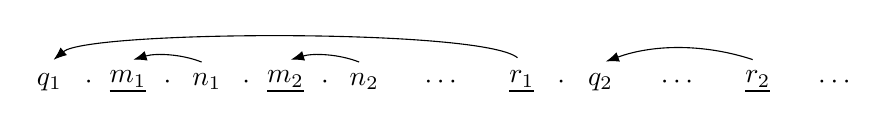
\begin{tikzpicture}[baseline=(current bounding box.center), yscale=0.6]
        \node (q1) at (0,0) {$q_1$};
        \node at (0.5,0) {$\cdot$};
        \node (m1) at (1,0) {$\underline{m_1}$};
        \node at (1.5,0) {$\cdot$};
        \node (n1) at (2,0) {$n_1$};
        \node at (2.5,0) {$\cdot$};
        \node (m2) at (3,0) {$\underline{m_2}$};
        \node at (3.5,0) {$\cdot$};
        \node (n2) at (4,0) {$n_2$};
        \node (dots) at (5,0) {$\cdots$};
        \node (r1) at (6,0) {$\underline{r_1}$};
        \node at (6.5,0) {$\cdot$};
        \node (q2) at (7,0) {$q_2$};
        \node at (8,0) {$\cdots$};
        \node (r2) at (9,0) {$\underline{r_2}$};
        \node (rest) at (10,0) {$\cdots$};

        \draw[{Latex}-, shorten <=2pt, shorten >=2pt] (q1.north).. controls +(0.5cm, 0.7cm) and +(-0.5cm, 0.7cm) .. (r1.north);
        \draw[{Latex}-, bend left=30, shorten <=2pt, shorten >=2pt] (m1.north) to (n1.north);
        \draw[{Latex}-, bend left=30, shorten <=2pt, shorten >=2pt] (m2.north) to (n2.north);
        \draw[{Latex}-, bend left=30, shorten <=2pt, shorten >=2pt] (q2.north) to (r2.north);
      \end{tikzpicture}
    \]
    \\[-1em]
    where $q_i \in F$ are the events triggered by the environment,
    and the component triggers events $m_i \in E$.
    \\[1em]
    A strategy $\sigma : E \rightarrow F$
    is a prefix-closed set of plays.
  \end{definition}
  \pause
  \begin{example}[Top-level and intermediate specifications]
    The strategies
    $\Gamma_\kw{hello},
    \Gamma_\kw{secret},
    \Gamma_\kw{decode} : \mathcal{S} \rightarrow \mathcal{P}$
    specify the corresponding commands.
    {\footnotesize
      \begin{gather*}
        \Gamma_\kw{hello} \: \vDash \: \kw{run}
        \cdot
        \underline{\kw{write}_1[\texttt{\textnormal{"hello, world!\textbackslash{}n"}}] }
        \cdot 14
        \cdot \underline{0}
        \qquad
        \Gamma_\kw{secret} \: \vDash \: \kw{run}
        \cdot
        \underline{\kw{write}_1[\texttt{\textnormal{"uryyb, jbeyq!\textbackslash{}n"}}] }
        \cdot 14
        \cdot \underline{0}
        \\
        \Gamma_\kw{decode} \: \vDash \: \kw{run} \cdot
        \underline{\kw{read}_0[100]} \cdot
        \texttt{\textnormal{"uryyb, jbeyq!\textbackslash{}n"}} \cdot
        \underline{\kw{write}_1[\texttt{\textnormal{"hello, world!\textbackslash{}n"}}]} \cdot
        14 \cdot
        \underline{0}
      \end{gather*}
    }
    \vspace{-2ex}
    \[
      \Gamma_\kw{hello} \subseteq \Gamma_\kw{secret} \mid \Gamma_\kw{decode}
    \]
  \end{example}
\end{frame}

\begin{frame}[fragile]{Layered Composition}
  The stragies $\sigma_1 : F \rightarrow G$ and
  $\sigma_2 : E \rightarrow F$ can be composed to obtain:
  \[
    \sigma_1 \odot \sigma_2 : E \rightarrow G
  \]
  \pause
  This is done by letting them interact over $F$
  in the following way:
  \[
    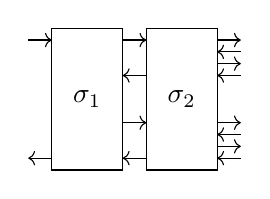
\begin{tikzpicture}[yscale=0.15,xscale=0.30]
      \draw (1,-1) rectangle (4,11) node[midway] {$\sigma_1$};
      \draw (5,-1) rectangle (8,11) node[midway] {$\sigma_2$};
      %\draw (5,-1) rectangle (8,4) node[midway] {$L_2$};
      \draw[->] (0,10) -- (1,10);
      \draw[->] (4,10) -- (5,10);
      \draw[->] (8,10) -- (9,10);
      \draw[->] (9,9) -- (8,9);
      \draw[->] (8,8) -- (9,8);
      \draw[->] (9,7) -- (8,7);
      \draw[->] (5,7) -- (4,7);
      \draw[->] (4,3) -- (5,3);
      \draw[->] (8,3) -- (9,3);
      \draw[->] (9,2) -- (8,2);
      \draw[->] (8,1) -- (9,1);
      \draw[->] (9,0) -- (8,0);
      \draw[->] (5,0) -- (4,0);
      \draw[->] (1,0) -- (0,0);
    \end{tikzpicture}
  \]
  \pause
  \begin{example}[Letting two C components interact]
    We can describe what happens
    when we let $\kw{decode.c}$ call into $\kw{rot13.c}$ as:
    \[
      \kw{Clight}(\kw{decode.c}) \odot \kw{Clight}(\kw{rot13.c})
      \::\: \mathcal{C} \at \kw{mem} \rightarrow
      \mathcal{C} \at \kw{mem}
    \]
    They connect over a common interface $\mathcal{C}\at\kw{mem}$:
    \[
      \mathcal{C} \at \kw{mem}
      \xrightarrow{\kw{Clight}(\kw{rot13.c})}
      \mathcal{C} \at \kw{mem}
      \xrightarrow{\kw{Clight}(\kw{decode.c})}
      \mathcal{C} \at \kw{mem}
    \]
  \end{example}
  %  \begin{example}[Assembly linking]
  %    %To let $\kw{secret.s}$ call into $\kw{rot13.s}$ we can compute:
  %    %\[ \kw{Asm}(\kw{secret.s}) \odot \kw{Asm}(\kw{rot13.s}) \]
  %    A key ingredient in our example is
  %    the assembly linking theorem:
  %    \[ \ell \::\:
  %       \kw{Asm}(\kw{secret.s}) \odot \kw{Asm}(\kw{rot13.s}) \:\le\:
  %       \kw{Asm}(\kw{secret.s} + \kw{rot13.s}) \]
  %    The two strategies synchronize over $\kw{rot13()}$ calls,
  %    which become hidden internal calls.
  %  \end{example}

\end{frame}

\begin{frame}{Flat Composition}
  Strategies can also be composed ``side by side'':
  \begin{itemize}
    \item Effect signatures compose as $E_1 \oplus E_2$ (direct sum);
    \item Strategies compose as $\sigma_1 \oplus \sigma_2 : E_1 \oplus E_2 \rightarrow F_1 \oplus F_2$.
  \end{itemize}
  \pause
  \begin{example}[Per-file interfaces]
    $\kw{read}$ and $\kw{write}$ to a particular file descriptor:
    \[
      \mathcal{F} := \{ \kw{read}[n] : \Sigma^*,\ \kw{write}[s] : \mathbb{N}
      \mid n \in \mathbb{N}, s \in \Sigma^* \}
    \]
    We can focus on $\kw{read}$ and $\kw{write}$ to $\kw{stdin}$ and $\kw{stdout}$:
    \[
      \mathcal{S} := \mathcal{F} \oplus \mathcal{F}
    \]
  \end{example}

\end{frame}

\begin{frame}[fragile]{Pipe Operator}
  \begin{itemize}
    \item Scheduler $\kw{seq}: \mathcal{P} \oplus \mathcal{P} \rightarrow \mathcal{P}$
      \[
        \kw{seq} \vDash
        \kw{run}
        \cdot \underline{\kw{run}_1} \cdot n
        \cdot \underline{\kw{run}_2} \cdot m
        \cdot \underline{m}
      \]
      \pause
    \item FIFO buffer $\kw{fifo}: \mathbf{0} \rightarrow \mathcal{F} \oplus \mathcal{F}$
      \parbox{\linewidth}{
        {\small
          \[
            \kw{fifo} \: \vDash \:
            (\kw{write_0}[\texttt{"hello, "}] \ \cdot \ \underline{7}) \ \cdot\
            (\kw{write_0}[\texttt{"world!\textbackslash{}n"}] \ \cdot\  \underline{7}) \ \cdot\
            (\kw{read_1}[100] \ \cdot\  \underline{\texttt{"hello, world!\textbackslash{}n"}})
      \]}}
      \pause
    \item Definition of pipe operator:
  \end{itemize}
  \[
    P \mid Q \: := \:
    \kw{seq} \odot (P \oplus Q)
    \odot (\mathcal{F} \oplus \kw{fifo} \oplus \mathcal{F})
  \]

  \begin{center}
    \resizebox{0.5\linewidth}{!}{
      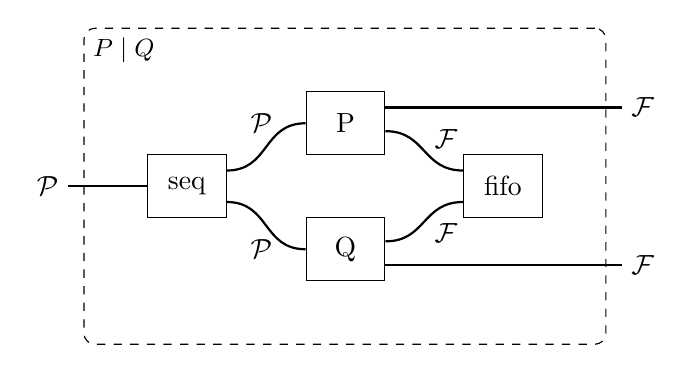
\begin{tikzpicture}[
          box/.style = {draw, minimum width=10mm, minimum height=8mm, align=center},
          wire/.style = {thick},
          dot/.style  = {circle, fill, inner sep=1.3pt}
        ]

        % --- blocks
        \node[box]                                  (seq)  {seq};
        \node[box, right=10mm of seq, yshift= 8mm]  (P)    {P};
        \node[box, right=10mm of seq, yshift=-8mm]  (Q)    {Q};
        \node[box, right=30mm of seq]               (fifo) {fifo};
        \node[right=30mm of P, yshift= 2mm]         (Px)   {$\mathcal{F}$};
        \node[right=30mm of Q, yshift=-2mm]         (Qx)   {$\mathcal{F}$};
        \node[left=10mm of seq]                     (Sx)   {$\mathcal{P}$};
        \node[left=3mm of P]                        (Pl)   {$\mathcal{P}$};
        \node[left=3mm of Q]                        (Ql)   {$\mathcal{P}$};
        \node[right=5mm of P, yshift=-2mm]          (Pr)   {$\mathcal{F}$};
        \node[right=5mm of Q, yshift=+2mm]          (Qr)   {$\mathcal{F}$};

        % convenient left/right x positions for long wires

        \coordinate (TopL) at ($(seq.north)+(0,8mm)$);
        \coordinate (TopR) at ($(fifo.north)+(0,8mm)$);
        \coordinate (BotL) at ($(seq.south)+(0,-8mm)$);
        \coordinate (BotR) at ($(fifo.south)+(0,-8mm)$);

        % --- internal wiring
        \draw[wire] (Sx) -- (seq.west);
        \draw[wire] (seq.east)+(0,2mm) to[out=0,in=180,looseness=1.2] (P.west);
        \draw[wire] (seq.east)+(0,-2mm) to[out=0,in=180,looseness=1.2] (Q.west);
        \draw[wire] (P.east)+(0,-1mm) to[out=0,in=180,looseness=1.2] ($(fifo.west)+(0,+2mm)$);
        \draw[wire] (Q.east)+(0,+1mm) to[out=0,in=180,looseness=1.2] ($(fifo.west)+(0,-2mm)$);
        \draw[wire] (P.east)+(0,+2mm) -- (Px);
        \draw[wire] (Q.east)+(0,-2mm) -- (Qx);

        % --- dashed enclosure with label
        \node[
          fit=(seq)(P)(Q)(fifo)(TopL)(TopR)(BotL)(BotR),
          draw, dashed, rounded corners, inner sep=8mm,
          label={[anchor=north west]north west:{\small $P \mid Q$}}
        ] {};
    \end{tikzpicture}}
  \end{center}

\end{frame}

\begin{frame}{CompCertO}
  \begin{columns}[onlytextwidth,T]
    \begin{column}{0.6\textwidth}
      \begin{itemize}
        \item Language interfaces $\mathcal{C}$, $\mathcal{A}$, $\mathcal{M}$, $\mathcal{L}$
        \item Labeled transition system
          \begin{align*}
            \kw{Clight}(\kw{p.c}) &: \mathcal{C}\at\kw{mem} \twoheadrightarrow \mathcal{C}\at\kw{mem}\\
            \kw{Asm}(\kw{p.s}) &: \mathcal{A}\at\kw{mem} \twoheadrightarrow \mathcal{A}\at\kw{mem}
          \end{align*}
        \item Forward simulation with simulation convention
          \[
            \kw{Clight}(\kw{p.c}) \le_{\mathbb{C} \twoheadrightarrow \mathbb{C}} \kw{Asm}(\kw{p.s})
          \]
          where
          $\mathbb{C} : \mathcal{C}\at\kw{mem} \Leftrightarrow \mathcal{A}\at\kw{mem}$
      \end{itemize}
    \end{column}
    \begin{column}{0.4\textwidth}
      \resizebox{0.75\linewidth}{!}{
        \setlength\tabcolsep{0.25ex}%
        \centering\scriptsize
        \begin{tabular}{lrclr}
          Language/Pass &
          \multicolumn{3}{c}{\hspace{-1.7em}Conventions}
          \\[1ex]
          \rowcolor{ACMLightBlue}
          \textbf{Clight} &
          $\mathcal{C}$ &
          $\twoheadrightarrow$ &
          $\mathcal{C}$
          \\
          \kw{SimplLocals} &
          $\kw{injp}$ &
          $\twoheadrightarrow$ &
          $\kw{inj}$
          \\
          \kw{Cshmgen} &
          \kw{id} &
          $\twoheadrightarrow$ &
          \kw{id}
          \\
          \rowcolor{ACMLightBlue}
          \textbf{Csharpminor} &
          $\mathcal{C}$ &
          $\twoheadrightarrow$ &
          $\mathcal{C}$
          \\
          \kw{Cminorgen} &
          $\kw{injp}$ &
          $\twoheadrightarrow$ &
          $\kw{inj}$
          \\
          \rowcolor{ACMLightBlue}
          \textbf{Cminor} &
          $\mathcal{C}$ &
          $\twoheadrightarrow$ &
          $\mathcal{C}$
          \\
          \kw{Selection} &
          $\kw{wt} \cdot \kw{ext}$ &
          $\twoheadrightarrow$ &
          $\kw{wt} \cdot \kw{ext}$
          \\
          \rowcolor{ACMLightBlue}
          \textbf{CminorSel} &
          $\mathcal{C}$ &
          $\twoheadrightarrow$ &
          $\mathcal{C}$
          \\
          \kw{RTLgen} &
          $\kw{ext}$ &
          $\twoheadrightarrow$ &
          $\kw{ext}$
          \\
          \rowcolor{ACMLightBlue}
          \textbf{RTL} &
          $\mathcal{C}$ &
          $\twoheadrightarrow$ &
          $\mathcal{C}$
          \\
          $\kw{Tailcall}$ &
          $\kw{ext}$ &
          $\twoheadrightarrow$ &
          $\kw{ext}$
          \\
          \kw{Inlining} &
          $\kw{injp}$ &
          $\twoheadrightarrow$ &
          $\kw{inj}$
          \\
          \kw{Renumber} &
          $\kw{id}$ &
          $\twoheadrightarrow$ &
          $\kw{id}$
          \\
          $\kw{Constprop}$ &
          $\kw{va} \cdot \kw{ext}$ &
          $\twoheadrightarrow$ &
          $\kw{va} \cdot \kw{ext}$
          \\
          $\kw{CSE}$ &
          $\kw{va} \cdot \kw{ext}$ &
          $\twoheadrightarrow$ &
          $\kw{va} \cdot \kw{ext}$
          \\
          $\kw{Deadcode}$ &
          $\kw{va} \cdot \kw{ext}$ &
          $\twoheadrightarrow$ &
          $\kw{va} \cdot \kw{ext}$
          %\st{Unusedglob} \\
          \\
          \kw{Allocation} &
          \hspace{-2em} $\kw{wt} \cdot \kw{ext} \cdot \kw{CL} $ &
          $\twoheadrightarrow$ &
          $\kw{wt} \cdot \kw{ext} \cdot \kw{CL}$
          \\
          \rowcolor{ACMBlue}
          \textbf{LTL} &
          $\mathcal{L}$ &
          $\twoheadrightarrow$ &
          $\mathcal{L}$
          \\
          \kw{Tunneling} &
          $\kw{ext}$ &
          $\twoheadrightarrow$ &
          $\kw{ext}$
          \\
          \kw{Linearize} &
          \kw{id} &
          $\twoheadrightarrow$ &
          \kw{id}
          \\
          \rowcolor{ACMBlue}
          \textbf{Linear} &
          $\mathcal{L}$ &
          $\twoheadrightarrow$ &
          $\mathcal{L}$
          \\
          \kw{CleanupLabels} &
          \kw{id} &
          $\twoheadrightarrow$ &
          \kw{id}
          \\
          \kw{Debugvar} &
          \kw{id} &
          $\twoheadrightarrow$ &
          \kw{id}
          \\
          \kw{Stacking} &
          $\kw{injp} \cdot \kw{LM} $ &
          $\twoheadrightarrow$ &
          $\kw{LM} \cdot \kw{inj}$
          \\
          \rowcolor{ACMOrange}
          \textbf{Mach} &
          $\mathcal{M}$ &
          $\twoheadrightarrow$ &
          $\mathcal{M}$
          \\
          \kw{Asmgen} &
          $\kw{ext} \cdot \kw{MA}$ &
          $\twoheadrightarrow$ &
          $\kw{ext} \cdot \kw{MA}$
          \\
          \rowcolor{ACMRed}
          \textbf{Asm} &
          $\mathcal{A}$ &
          $\twoheadrightarrow$ &
          $\mathcal{A}$
          %\\
          %\midrule
          %\multicolumn{4}{r}{\bf Total \quad{} } &
          %  \bf +1{,}136 & \bf (+3\%)
          %\\
        \end{tabular}
      }
    \end{column}
  \end{columns}

\end{frame}

\begin{frame}{Integration with CompCertO---Embedding}
  A CompCertO transition system $L : A \twoheadrightarrow B$
  can be embedded into a strategy
  \[
    \llbracket L \rrbracket : \llbracket A \rrbracket \rightarrow \llbracket B \rrbracket
    \vspace{-2ex}
  \]
  \pause
  \begin{theorem}[Compatibility with composition]
    The embedding from CompCertO semantics into strategies preserves composition:
    \vspace{-1ex}
    \[
      \llbracket L_1 \rrbracket
      \odot
      \llbracket L_2 \rrbracket
      \subseteq
      \llbracket L_1 \odot L_2 \rrbracket
    \]
  \end{theorem}
  \pause
  \begin{theorem}[Linking property]
    For assembly-level transition systems:
    \vspace{-1ex}
    \begin{align*}
      \llbracket \kw{Asm}(\kw{p_1.s}) \rrbracket
      \odot
      \llbracket \kw{Asm}(\kw{p_2.s}) \rrbracket
      & \subseteq
      \llbracket \kw{Asm}(\kw{p_1.s}) \odot \kw{Asm}(\kw{p_2.s}) \rrbracket\\
      & \subseteq
      \llbracket \kw{Asm}(\kw{p_1.s}) \oplus \kw{Asm}(\kw{p_2.s}) \rrbracket\\
      & \subseteq
      \llbracket \kw{Asm}(\kw{p_1.s} + \kw{p_2.s}) \rrbracket
    \end{align*}
  \end{theorem}
\end{frame}

\begin{frame}{Integration with CompCertO---Loader}
  Loaders turn open semantics in CompCertO into standalone processes.
  \begin{gather*}
    \kw{entry}_\A : \A \rightarrow \mathcal{P} \qquad
    \kw{runtime}_\A : \mathcal{S} \rightarrow \A \\
    \kw{entry}_\C : \C \rightarrow \mathcal{P} \qquad
    \kw{runtime}_\C : \mathcal{S} \rightarrow \C\\
    \kw{load}_\A(L : \A \twoheadrightarrow \A) : \mathcal{S} \rightarrow \mathcal{P} \::=\: \kw{entry}_\A \odot L \odot \kw{runtime}_\A \\
    \kw{load}_\C(L : \C \twoheadrightarrow \C) : \mathcal{S} \rightarrow \mathcal{P} \::=\: \kw{entry}_\C \odot L \odot \kw{runtime}_\C
  \end{gather*}
  \pause
  The $\kw{entry}_\mathcal{A}$ invokes the main function
  following the assembly-level convention:
  \[
    \kw{entry}_\mathcal{A} \:\vDash\:
    \kw{run} \cdot
    \underline{\vec{rs_0}[\kw{PC}\mapsto \kw{main},
        \kw{RA} \mapsto \kw{null},
    \kw{RSP}\mapsto \kw{null}]@m_0} \cdot
    \vec{rs}[\kw{RAX} \mapsto r]@m \cdot \underline{r}
    \vspace{-2ex}
  \]
  \pause
  \begin{theorem}[Loader simulation]
    Simulation in CompCertO implies simple refinement in the process behavior:
    \begin{center}
      \begin{prooftree}
        \hypo{L_1 \le_{\mathbb{C} \rightarrow \mathbb{C}} L_2}
        \infer1{\kw{load}_\mathcal{C}(\llbracket L_1 \rrbracket) \subseteq
        \kw{load}_\mathcal{A}(\llbracket L_2 \rrbracket)}
      \end{prooftree}
    \end{center}
  \end{theorem}
\end{frame}

\begin{frame}
  \resizebox{\textwidth}{0.45\textheight}{
    \begin{minipage}{\textwidth}
      \begin{align}
        \Gamma_\kw{decode}
        & \subseteq \kw{load}_\C(\Sigma_\kw{decode})
        \tag{(1) by manual proof}\\
        & \subseteq \kw{load}_\C(\llbracket \kw{Clight}(\kw{decode.c}) \rrbracket
        \odot \llbracket \kw{Clight}(\kw{rot13.c}) \rrbracket)
        \tag{(2) by manual proof}\\
        & \subseteq \kw{load}_\C(\llbracket \kw{Clight}(\kw{decode.c})
        \odot \kw{Clight}(\kw{rot13.c}) \rrbracket)
        \tag{(3) by property of embedding}\\
        & \subseteq \kw{load}_\mathcal{A}(\llbracket \kw{Asm}(\kw{decode.s})
        \odot \kw{Asm}(\kw{rot13.s}) \rrbracket)
        \tag{(4) by loader simulation and compiler correctness}\\
        & \subseteq \kw{load}_\mathcal{A}(\llbracket \kw{Asm}(\kw{decode.s} + \kw{rot13.s}) \rrbracket)
        \tag{(5) by CompCertO's linking property}\\
        \Gamma_\kw{secret}
        & \subseteq \kw{load}_\C(\Sigma_\kw{secret})
        \tag{(6) by manual proof}\\
        & \subseteq \kw{load}_\C(\llbracket L_\kw{secret} \rrbracket
        \odot \llbracket \kw{Clight}(\kw{rot13.c}) \rrbracket)
        \tag{(7) by manual proof}\\
        & \subseteq \kw{load}_\C(\llbracket L_\kw{secret}
        \odot \kw{Clight}(\kw{rot13.c}) \rrbracket)
        \tag{(8) by property of embedding}\\
        & \subseteq \kw{load}_\mathcal{A}(\llbracket \kw{Asm}(\kw{secret.s})
        \odot \kw{Asm}(\kw{rot13.s}) \rrbracket)
        \tag{(9) by loader simulation and manual proof}
        \\
        & \subseteq \kw{load}_\mathcal{A}(\llbracket \kw{Asm}(\kw{secret.s} + \kw{rot13.s}) \rrbracket)
        \tag{(10) by CompCertO's linking property}
        \\
        \Gamma_\kw{hello}
        & \subseteq \Gamma_\kw{secret} \mid \Gamma_\kw{decode}
        \tag{(11) by manual proof}\\
        & \subseteq \kw{load}_\mathcal{A}(\kw{Asm}(\kw{secret.s} + \kw{rot13.s}))
        \mid \kw{load}_\mathcal{A}(\kw{Asm}(\kw{decode.s} + \kw{rot13.s}))
        \tag{(12) by monotonicity}
      \end{align}
    \end{minipage}
  }
\end{frame}

\subsection{Refinement Conventions and Refinement Squares}

\begin{frame}{Generalizing Refinement}
  Simple notion of refinement:
  \[
    \sigma_1 \subseteq \sigma_2 : E \rightarrow F
  \]
  Any behavior exhibited by $\sigma_1$ must be also exhibited by $\sigma_2$.
  \\[3ex]
  Generalizing this to different effect signatures:
  \begin{align*}
    \sigma_1 : E_1 \rightarrow F_1 & \vDash q_1 \cdot \underline{m_1} \cdot n_1 \cdots \underline{r_1} \cdots \\
    \sigma_2 : E_2 \rightarrow F_2 & \vDash q_2 \cdot \underline{m_2} \cdot n_2 \cdots \underline{r_2} \cdots
  \end{align*}
\end{frame}

\begin{frame}[fragile]{Duality of Choices}
  Consider:
  \begin{columns}
    \begin{column}{.5\textwidth}
      \begin{gather*}
        \sigma_1 : E_1 \rightarrow F_1 \vDash q_1 \cdot \underline{m_1} \cdot n_1 \cdots \underline{r_1} \cdots \\
        \sigma_2 : E_2 \rightarrow F_2 \vDash q_2 \cdot \underline{m_2} \cdot n_2 \cdots \underline{r_2} \cdots\\
      \end{gather*}
    \end{column}
    \begin{column}{.35\textwidth}
      \begin{gather*}
        \mathbf{R} : E_1 \leftrightarrow E_2 \\
        \mathbf{S} : F_1 \leftrightarrow F_2\\
      \end{gather*}
    \end{column}
  \end{columns}
  \pause
  \begin{columns}
    \begin{column}{.5\textwidth}
      \visible<2->{
      When $\sigma_1$ makes the question $\underline{m_1}$,}
      \begin{center}
        \begin{tikzcd}
          \only<2->{
          \sigma_1 \ar[r,dash] \ar[d, dash]} &
          \only<2->{\underline{m_1}
          \ar[d,dash,dashed,"\mathbf{R}^\circ"']} \\
          \only<2->{\sigma_2 \ar[r,dashed,dash]} &
          \only<2->{\exists \: \underline{m_2}}
        \end{tikzcd}
      \end{center}
      \visible<4->{
      For incoming question, $q_2$ is chose by client,}
      \begin{center}
        \begin{tikzcd}
          \only<4->{
          \sigma_1 \ar[r,dash] \ar[d, dash]} &
          \only<4->{q_1
          \ar[d,dash,dashed,"\mathbf{S}^\circ"']} \\
          \only<4->{\sigma_2 \ar[r,dashed,dash]} &
          \only<4->{\forall \: q_2}
        \end{tikzcd}
      \end{center}
    \end{column}
    \begin{column}{.52\textwidth}
      \visible<3->{
      When $\sigma_1$ returns the answer $\underline{r_1}$,}
      \begin{center}
        \begin{tikzcd}
          \only<3->{
          \sigma_1 \ar[r,dash] \ar[d, dash]} &
          \only<3->{\underline{r_1}
          \ar[d,dash,dashed,"\mathbf{S}^\bullet"']} \\
          \only<3->{\sigma_2 \ar[r,dashed,dash]} &
          \only<3->{\exists \: \underline{r_2}}
        \end{tikzcd}
      \end{center}
      \visible<5->{
      For incoming answer, $n_2$ is chose by handler,}
      \begin{center}
        \begin{tikzcd}
          \only<5->{
          \sigma_1 \ar[r,dash] \ar[d, dash]} &
          \only<5->{n_1
          \ar[d,dash,dashed,"\mathbf{R}^\bullet"']} \\
          \only<5->{\sigma_2 \ar[r,dashed,dash]} &
          \only<5->{\forall \: n_2}
        \end{tikzcd}
      \end{center}

    \end{column}
  \end{columns}
\end{frame}

\begin{frame}{Alternating Quantifiers}
  Consider:
  \begin{columns}
    \begin{column}{.5\textwidth}
      \begin{gather*}
        \sigma_1 : E_1 \rightarrow F_1 \vDash q_1 \cdot \underline{m_1} \cdot n_1 \cdots \underline{r_1} \cdots \\
        \sigma_2 : E_2 \rightarrow F_2 \vDash q_2 \cdot \underline{m_2} \cdot n_2 \cdots \underline{r_2} \cdots\\
      \end{gather*}
    \end{column}
    \begin{column}{.35\textwidth}
      \begin{gather*}
        \mathbf{R} : E_1 \leftrightarrow E_2 \\
        \mathbf{S} : F_1 \leftrightarrow F_2\\
      \end{gather*}
    \end{column}
  \end{columns}
  Based on the intuition,
  the refinement property is (informally) stated as:
  \begin{alignat*}
    \forall \forall q_1, \underline{m_1}, q_2,& \ \ q_1 \cdot \underline{m_1} \in \sigma_1
    && \ \wedge\  q_1 \mathrel{\mathbf{S}^\que} q_2 \rightarrow \\
    \exists \underline{m_2},& \ \ q_2 \cdot \underline{m_2} \in \sigma_2
    && \ \wedge\  \underline{m_1} \mathrel{\mathbf{R}^\circ} \underline{m_2}
    \ \wedge\ \\
    \forall n_1, \underline{m'_1}, n_2,& \ \ n_1 \cdot \underline{m'_1} \in (q_1 \cdot \underline{m_1} \backslash \sigma_1)
    && \ \wedge\  n_1 \mathrel{\mathbf{R}^\bullet_{m_1m_2}} n_2 \rightarrow \\
    \exists \underline{m'_2},& \ \ n_2 \cdot \underline{m'_2} \in (q_2 \cdot \underline{m_2} \backslash \sigma_2)
    && \ \wedge\  \underline{m'_1} \mathrel{\mathbf{R}^\que_{m_1m_2n_1n_2}} \underline{m'_2}
    \ \wedge\ \\
    & \cdots && \\
    & \cdots &&
  \end{alignat*}
\end{frame}

\begin{frame}{Refinement Conventions}
  \begin{definition}[Refinement Conventions]
    Refinement conventions of type $\mathbf{R} : E \leftrightarrow F$
    are constructed using plays of the form
    \[
      s \in P_{E \leftrightarrow F} \: ::= \:
      \visible<2->{(m_1, m_2) \bot \: \mid \:}
      (m_1, m_2) (n_1, n_2) \, s \visible<2->{\: \mid \:
      (m_1, m_2) (n_1, n_2) \top}
    \]
    \vspace{-2ex}
  \end{definition}
  For example,
  \begin{align*}
    \mathbf{R}_\kw{queue} : E_\kw{bq} \leftrightarrow E_\kw{bq} \at [V] \vDash\
    & \bigl(\kw{enq}(v_1),\kw{enq}(v_1)\at \kw{nil}\bigr)
    \bigl(*, * \at [v_1]\bigr)\\[1ex]
    & \bigl(\kw{enq}(v_2),\kw{enq}(v_2)\at [v_1]\bigr)
    \bigl(*, * \at [v_1, v_2]\bigr)\\[1ex]
    & \bigl(\kw{deq},\kw{deq}\at [v_1, v_2]\bigr)
    \bigl(v_1, v_1 \at [v_2]\bigr)\\[1ex]
    & \cdots
  \end{align*}
  \pause
  \vspace{-4ex}
  \begin{itemize}
    \item $(m_1, m_2) \bot$ allows the questions $m_1$ and $m_2$
    \item $(m_1, m_2) (n_1, n_2) \top$ disallows the pair
      $n_1$ and $n_2$ as related answers
  \end{itemize}
\end{frame}

\begin{frame}{Ordering Refinement Conventions}
  \begin{itemize}
    \item $(m_1, m_2) \bot$ allows the questions $m_1$ and $m_2$
    \item $(m_1, m_2) (n_1, n_2) \top$ disallows the pair
      $n_1$ and $n_2$ as related answers
  \end{itemize}
  \vspace{1ex}
  \[
    m_1 \mathrel{\mathbf{R}^\circ} m_2 \::\Leftrightarrow\:
    (m_1, m_2)\bot \in \mathbf{R}
    \qquad
    n_1 \mathrel{\mathbf{R}^\bullet_{m_1m_2}} n_2 \::\Leftrightarrow\:
    (m_1, m_2)(n_1, n_2)\top \notin \mathbf{R}
    \vspace{4ex}
  \]

  \pause
  Refinement conventions are downward closed sets of such plays ordered by:
  {\small
    \[
      s_1 \preceq s_2 \:\Longrightarrow\:
      (m_1, m_2) \bot \:\preceq\:
      (m_1, m_2) (n_1, n_2) s_1 \:\preceq\:
      (m_1, m_2) (n_1, n_2) s_2 \:\preceq\:
      (m_1, m_2) (n_1, n_2) \top
  \]}

  $\mathbf{R} \subseteq \mathbf{R'}$ when
  $\mathbf{R'}$ admits more pairs of questions
  and less pairs of answers (roughly).
\end{frame}

\begin{frame}[fragile]{Refinement Conventions in a Refinement Square}
  In a refinement square
  $
  \begin{tikzcd}[sep=small]
    E_1
    \ar[rr, "\sigma"] \ar[dd, leftrightarrow, "\mathbf{R}"]
    && F_1
    \ar[dd, leftrightarrow, "\mathbf{S}"]
    \\
    & \phi &
    \\
    E_2 \ar[rr, "\tau"] && F_2
  \end{tikzcd}
  $
  \\[1ex]
  \begin{columns}
    \begin{column}{.5\textwidth}
      As a client, it gets easier to prove when
      \begin{itemize}
        \item $\mathbf{R}$ admits more pairs of questions
        \item $\mathbf{R}$ admits less pairs of answers
      \end{itemize}
    \end{column}
    \visible<3->{
      \begin{column}{.5\textwidth}
        As a handler, it gets easier to prove when
        \begin{itemize}
          \item $\mathbf{S}$ admits less pairs of questions
          \item $\mathbf{S}$ admits more pairs of answers
        \end{itemize}
      \end{column}
    }
  \end{columns}
  \vspace{2ex}
  Therefore,
  \[
    \begin{tikzcd}[sep=small]
      \only<2->{E_1}
      \only<2->{\ar[rr, rightarrow, "\kw{id}"]}
      \only<2->{\ar[dd, leftrightarrow, "\mathbf{R'}"']}
      && \only<2->{E_1}
      \only<2->{\ar[rr, "\sigma"] \ar[dd, leftrightarrow, "\mathbf{R}"]}
      && \only<2->{F_1}
      \only<4->{\ar[rr, rightarrow, "\kw{id}"]}
      \only<2->{\ar[dd, leftrightarrow, "\mathbf{S}"']}
      && \only<4->{F_1}
      \only<4->{\ar[dd, leftrightarrow, "\mathbf{S'}"]}
      \\
      & \only<2->{\mathbf{R} \subseteq \mathbf{R'}} && \only<2->{\phi} && \only<4->{\mathbf{S'} \subseteq \mathbf{S}}
      \\
      \only<2->{E_2}
      \only<2->{\ar[rr, rightarrow, "\kw{id}"]}
      && \only<2->{E_2 \ar[rr, "\tau"]} &&
      \only<2->{F_2}
      \only<4->{\ar[rr, rightarrow, "\kw{id}"]}
      && \only<4->{F_2}
    \end{tikzcd}
  \]

\end{frame}

\subsection{Spatial Composition and State Encapsulation}

\begin{frame}{Spatial Composition}
  The third composition principle is \textbf{spatial composition} $\at$,
  which acts on:
  \pause
  \begin{itemize}
    \item Effect signatures
      \[
        E \at U := \{ m @ u \mathbin: N \times U \mid
        m\mathbin:N \in E, \, u \in U \}
        \vspace{-2ex}
      \]
      \pause
    \item Strategies
      \[
        \begin{prooftree}
          \hypo{\sigma : E \rightarrow F}
          \infer1{\sigma \at U : E \at U \rightarrow F \at U}
        \end{prooftree}
      \]
      pass the state through:
      % {\small
      %   \begin{equation*}
      %     \begin{prooftree}
      %       \hypo{
      %         \sigma \:\vDash\: q \ \cdot\
      %         \underline{m_1} \ \cdot\ n_1 \ \cdot\
      %         \cdots
      %         \underline{m_n} \ \cdot\ n_n \ \cdot\
      %         \underline{r}
      %       }
      %       \infer1{
      %         \sigma \at U \:\vDash\: q\at u_0 \ \cdot\
      %         \underline{m_1\at u_0} \ \cdot\ n_1\at u_1 \ \cdot\
      %         \cdots \ \cdot\
      %         \underline{m_n\at u_{n-1}} \ \cdot\ n_n\at u_n \ \cdot\
      %         \underline{r\at u_n}
      %       }
      %     \end{prooftree}
      % \end{equation*}}
  \end{itemize}
  \begin{columns}
    \begin{column}{.5\textwidth}
      \[
        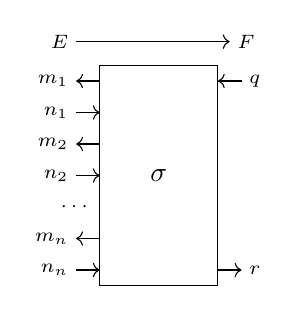
\begin{tikzpicture}[yscale=0.2,xscale=0.3]
          \draw (1,-1) rectangle (6,13) node[midway] {$\sigma$};
          \scriptsize
          \draw[<-] (0,12) node[left] {$m_1$} -- (1,12);
          \draw[<-] (6,12) -- (7,12) node[right] {$q$};
          \draw[->] (0,10) node[left] {$n_1$} -- (1,10) ;
          \draw[<-] (0,8) node[left] {$m_2$} -- (1,8);
          \draw[->] (0,6) node[left] {$n_2$} -- (1,6) ;
          \draw[<-] (0,2) node[left] {$m_n$} -- (1,2);
          \draw[<-] (7,0) node[right] {$r$} -- (6,0);
          \draw[<-] (1,0) -- (0,0) node[left] {$n_n$};
          \draw[->] (0,14.5) node[left] {$E$} -- (6.5,14.5) node[right] {$F$};
          \node at (0, 4) {$\cdots$};
        \end{tikzpicture}
      \]

    \end{column}
    \begin{column}{.5\textwidth}
      \[
        \hspace{-5em}
        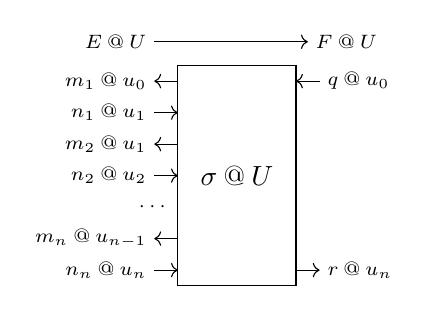
\begin{tikzpicture}[yscale=0.2,xscale=0.3]
          \draw (1,-1) rectangle (6,13) node[midway] {$\sigma\at U$};
          \scriptsize
          \draw[<-] (0,12) node[left] {$m_1\at u_0$} -- (1,12);
          \draw[<-] (6,12) -- (7,12) node[right] {$q\at u_0$};
          \draw[->] (0,10) node[left] {$n_1\at u_1$} -- (1,10);
          \draw[<-] (0,8) node[left] {$m_2\at u_1$} -- (1,8);
          \draw[->] (0,6) node[left] {$n_2\at u_2$} -- (1,6);
          \draw[<-] (0,2) node[left] {$m_n\at u_{n-1}$} -- (1,2);
          \draw[<-] (7,0) node[right] {$r \at u_n$} -- (6,0);
          \draw[<-] (1,0) -- (0,0) node[left] {$n_n \at u_n$};
          \draw[->] (0,14.5) node[left] {$E\at U$} -- (6.5,14.5) node[right] {$F\at U$};
          \node at (0, 4) {$\cdots$};
        \end{tikzpicture}
      \]
    \end{column}
  \end{columns}

\end{frame}

\begin{frame}{First Approach to State Encapsulation}
  Consider the strategy that implements queue operations
  \[
    \sigma_\kw{queue} : \mathbf{0} \rightarrow E_\kw{bq} \ \vDash\
    \kw{enq}(v_1)
    \ \cdot\ \underline{*}
    \ \cdot\ \kw{enq}(v_2)
    \ \cdot\ \underline{*}
    \ \cdot\ \kw{deq}
    \ \cdot\ \underline{v_1}
    \ \cdots
  \]
  \pause
  To define such a strategy,
  we can inductively define the plays in the strategy:
  \[
    \begin{prooftree}
      \infer0{\epsilon \in \sigma_{\kw{nil}} }
    \end{prooftree}
    \qquad
    \begin{prooftree}
      \hypo{s \in \sigma_{[v_2, \cdots]} }
      \infer1{\kw{deq} \cdot \underline{v_1} \cdot s \, \in \, \sigma_{[v_1, v_2, \cdots]} }
    \end{prooftree}
    \qquad
    \begin{prooftree}
      \hypo{s \in \sigma_{[v_1, v_2, \cdots, v]} }
      \infer1{\kw{enq}[v] \cdot \underline{*} \cdot s \, \in \, \sigma_{[v_1, v_2, \cdots]} }
    \end{prooftree}
  \]
  Here the state is retained from one execution to the next.
  \\[1em]
  \pause
  Then, $\sigma_\kw{queue}$ starts with the empty state:
  \[
    \sigma_\kw{queue} := \sigma_{\kw{nil}}
  \]

\end{frame}

\begin{frame}{Encapsulation Primitive}
  Generalizing the previous approach,
  we can define an encapsulation primitive
  \[\encap{u_0} : U \rightarrow \mathbf{1}\]
  for any state $u_0 \in U$ where $\mathbf{1}$
  only contains the dummy question and answer.
  \\[1em]
  \pause
  The encapsulation primitive can be composed
  with the identity strategy $\kw{id}: A \rightarrow A$:
  \[
    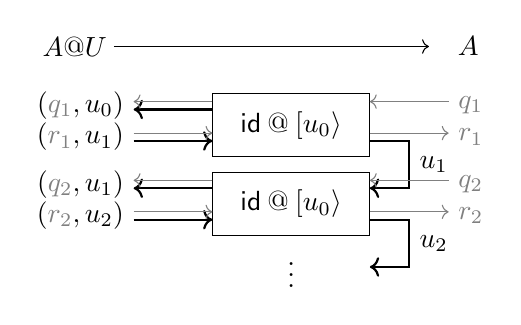
\begin{tikzpicture}[yscale=0.2,xscale=0.5]
      \begin{scope}
        \draw[fill=white] (0,0) rectangle (4,4) node[midway] {$\kw{id} \at \encap{u_0}$};
        \draw[fill=white] (0,5) rectangle (4,9) node[midway] {$\kw{id} \at \encap{u_0}$};
      \end{scope}
      \begin{scope}[thick]
        \draw[->] (0,8) -- (-2,8); % outgoing u0
        \draw[->] (-2,6) -- (0,6); % incoming u1
        \draw[->] (0,3) -- (-2,3); % outgoing u1
        \draw[->] (-2,1) -- (0,1); % incoming u2
      \end{scope}
      \begin{scope}[thick]
        \draw[->] (4,6) -- (5,6) -- node[right] {$u_1$} (5,3) -- (4,3);
        \draw[->] (4,1) -- (5,1) -- node[right] {$u_2$} (5,-2) -- (4,-2);
      \end{scope}
      \begin{scope}[yshift=0.25cm]
        \draw (6,8) node[right] {$\textcolor{gray}{q_1}$};
        \draw (-2,8) node[left] {$(\textcolor{gray}{q_1}, u_0)$};
        \draw (-2,6) node[left] {$(\textcolor{gray}{r_1}, u_1)$};
        \draw (6,6) node[right] {$\textcolor{gray}{r_1}$};
        \draw (6,3) node[right] {$\textcolor{gray}{q_2}$};
        \draw (-2,3) node[left] {$(\textcolor{gray}{q_2}, u_1)$};
        \draw (-2,1) node[left] {$(\textcolor{gray}{r_2}, u_2)$};
        \draw (6,1) node[right] {$\textcolor{gray}{r_2}$};
      \end{scope}
      \begin{scope}[gray,yshift=0.5cm]
        \draw[->] (6,8) -- (4,8); % incoming q1
        \draw[->] (0,8) -- (-2,8); % outgoing q1
        \draw[->] (-2,6) -- (0,6); % incoming r1
        \draw[->] (4,6) -- (6,6); % outgoing r1
        \draw[->] (6,3) -- (4,3); % incoming q2
        \draw[->] (0,3) -- (-2,3); % outgoing q2
        \draw[->] (-2,1) -- (0,1); % incoming r2
        \draw[->] (4,1) -- (6,1); % outgoing r2
      \end{scope}
      \begin{scope}
        \node at (2,-2) {$\vdots$};
        \node at (-3.5,12) {$A@U$};
        \node at (6.5,12) {$A$};
        \draw[->] (-2.5,12) -- (5.5,12);
      \end{scope}
    \end{tikzpicture}
  \]

  The state of the encapsulation primitive
  is never revealed to the environment.

\end{frame}

\begin{frame}[fragile]{Second Approach to State Encapsulation}

  We can first define a state-passing version of the queue:
  \begin{align*}
    \tau &\ :\ \mathbf{0} \rightarrow E_\kw{bq} \at [V]\\
    \tau &\ \vDash\
    \kw{enq}(v_1) \at \kw{nil} \ \cdot\
    \underline{* \at [v_1]} \ \cdot\
    \kw{enq}(v_2) \at [v_1] \ \cdot\
    \underline{* \at [v_1, v_2]} \ \cdot\
    \kw{deq} \at [v_1, v_2] \ \cdot\
    \underline{v_1 \at [v_2]}
  \end{align*}
  \pause
  and using the encapsulation primitive to recover the encapsulated queue as:
  \[
    \tau_\kw{nil} : \mathbf{0} \rightarrow E_\kw{bq} \::=\: (\kw{id}_{E_\kw{bq}} \at \encap{\kw{nil}}) \odot \tau
  \]

  \only<3->{The relation between the two approaches
  is shown in the following diagram:}
  \[
    \begin{tikzcd}[sep=small]
      \only<3->{\mathbf{0}}
      \only<3->{\ar[rr, "\sigma_\kw{nil}"]}
      \only<3->{\ar[dd, leftrightarrow, "="]}
      && \only<3->{E_\kw{bq}}
      \only<3->{\ar[rr, "\kw{id}"]}
      \only<3->{\ar[dd, leftrightarrow, "\mathbf{id} \at \encap{\kw{nil}}_*"]}
      && \only<3->{E_\kw{bq}}
      \only<3->{\ar[dd, leftrightarrow, "="]}
      \\
      & \only<3->{\psi_1} && \quad & \\
      \only<2->{\mathbf{0}}
      \only<2->{\ar[rr, "\tau"]}
      &&
      \only<2->{E_\kw{bq} \at [V]}
      \only<2->{\ar[rr, "\kw{id} \at \encap{\kw{nil}}"]}
      && \only<2->{E_\kw{bq}}
    \end{tikzcd}
  \]

  \only<3->{The square on the right is the conjoint property
  of the encapsulation primitive.}
\end{frame}

\begin{frame}[fragile]{Representation Independence}
  Two components may use different representations
  but otherwise exhibit identical behaviors.
  In this case,
  encapsulating their state will yield identical behaviors.
  \[
    \zeta : u \mathbin{R} v
    \quad\Longrightarrow\quad
    \encap{\zeta} : \encap{u} \le_{[R] \rightarrow \kw{id}_\mathbf{1}} \encap{v}
    \qquad
    \qquad
    \begin{tikzcd}[sep=tiny]
      U\ar[rr, "\encap{u}"] \ar[dd, leftrightarrow,"{[}R{]}"']
      && \mathbf{1} \ar[dd, leftrightarrow, "="] \\
      & \encap{\zeta} & \\
      V\ar[rr, "\encap{v}"'] && \mathbf{1}
    \end{tikzcd}
    \vspace{-5ex}
  \]
  \pause
  Continuing with the bounded queue example,
  \[
    \begin{tikzcd}[sep=small]
      \mathbf{0}
      \ar[rr, "\tau"]
      \ar[dd, leftrightarrow, "="]
      &&
      E_\kw{bq} \at [V]
      \ar[rr, "\kw{id} \at \encap{\kw{nil}}"]
      \ar[dd, leftrightarrow, "\mathbf{id} \at R"']
      && E_\kw{bq}
      \ar[dd, leftrightarrow, "="]
      \\
      & \psi_2 && \encap{\kw{nil} \mathbin{R} m_0} & \\
      \mathbf{0}
      \ar[rr, "\kw{Clight}"]
      && E_\kw{bq} \at \kw{mem}
      \ar[rr, "\kw{id} \at \encap{m_0}"]
      && E_\kw{bq}
    \end{tikzcd}
  \]
  where
  $R \subseteq [V] \times \kw{mem}$ is the refinement relation
  and $m_0 \in \kw{mem}$ is the initial memory state
  such that $\kw{nil} \mathbin{R} m_0$.

\end{frame}

\begin{frame}[fragile]{Putting All Together}
  \[
    \begin{tikzcd}[sep=small]
      \mathbf{0}
      \ar[rr, "\sigma_\kw{nil}"]
      \ar[dd, leftrightarrow, "="]
      && E_\kw{bq}
      \ar[rr, "\kw{id}"]
      \ar[dd, leftrightarrow, "\mathbf{id} \at \encap{\kw{nil}}_*"]
      && E_\kw{bq}
      \ar[dd, leftrightarrow, "="]
      \\
      & \psi_1 &&& \\
      \mathbf{0}
      \ar[rr, "\tau"]
      \ar[dd, leftrightarrow, "="]
      &&
      E_\kw{bq} \at [V]
      \ar[rr, "\kw{id} \at \encap{\kw{nil}}"]
      \ar[dd, leftrightarrow, "\mathbf{id} \at R"']
      && E_\kw{bq}
      \ar[dd, leftrightarrow, "="]
      \\
      & \psi_2 && \encap{\kw{nil} \mathbin{R} m_0} & \\
      \mathbf{0}
      \ar[rr, "\kw{Clight}"]
      && E_\kw{bq} \at \kw{mem}
      \ar[rr, "\kw{id} \at \encap{m_0}"]
      && E_\kw{bq}
    \end{tikzcd}
  \]
\end{frame}

\section{Application}

\subsection{ClightP Semantics}

\begin{frame}{ClightP Semantics}
  The motivation is to streamline the verification process between abstract state and concrete memory.
  \[
    \sigma_\kw{rb.c} : \mathbf{0} \rightarrow \C \at D_\kw{rb}
    \qquad
    \kw{Clight}(\kw{rb.c}) : \C \at \kw{mem} \rightarrow \C \at \kw{mem}
  \]
  \pause
  \begin{columns}
    \begin{column}{.6\textwidth}
      \begin{itemize}
        \item Directly translate the abstract state to detailed memory layout
        \item Must prove the rest of the memory is not modified
      \end{itemize}
    \end{column}
    \begin{column}{.4\textwidth}
      \begin{center}
        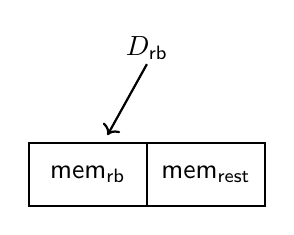
\begin{tikzpicture}
          \draw[thick] (0,0) rectangle (3,0.8);
          \draw[thick] (1.5,0) -- (1.5,0.8);
          \node at (0.75,0.4) {$\kw{mem}_\kw{rb}$};
          \node at (2.25,0.4) {$\kw{mem}_\kw{rest}$};
          \draw[->, thick] (1.5,1.8) -- (1,0.9);
          \node at (1.5,2) {$D_\kw{rb}$};
        \end{tikzpicture}
      \end{center}
    \end{column}
  \end{columns}
\end{frame}

\begin{frame}{ClightP Semantics}

  \begin{itemize}
    \item Extending Clight semantics with persistent environment
      \[
        \kw{ClightP}(M) : \C \at \kw{mem} \rightarrow \C \at \kw{mem} \at \kw{penv}
      \]
  \end{itemize}
  \vspace{-1em}
  \pause
  \begin{columns}
    \begin{column}{.7\textwidth}
      \begin{itemize}
        \item Translate the abstract state to persistent environment
        \item Compilation from ClightP to Clight automatically handles the persistent environment
        \item Encapsulate the persistent environment to keep it private
      \end{itemize}
    \end{column}
    \begin{column}{.3\textwidth}
      \begin{center}
        \hspace{-2em}
        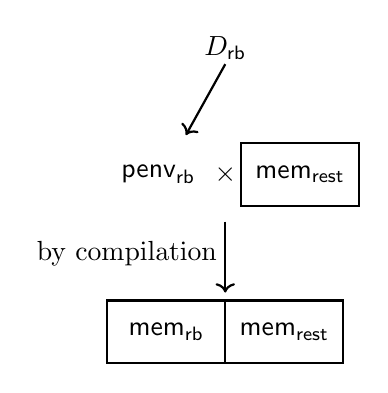
\begin{tikzpicture}
          \draw[thick] (0,0) rectangle (3,0.8);
          \draw[thick] (1.5,0) -- (1.5,0.8);
          \node at (0.75,0.4) {$\kw{mem}_\kw{rb}$};
          \node at (2.25,0.4) {$\kw{mem}_\kw{rest}$};
          \draw[->, thick] (1.5,3.8) -- (1,2.9);
          \node at (1.5,4) {$D_\kw{rb}$};
          \node at (0.65,2.4) {$\kw{penv}_\kw{rb}$};
          \node at (1.5,2.4) {$\times$};
          \node at (2.45,2.4) {$\kw{mem}_\kw{rest}$};
          \node at (0.25, 1.4) {by compilation};
          \draw[->, thick] (1.5,1.8) -- (1.5,0.9);
          \draw[thick] (1.7,2) rectangle (3.2,2.8);
        \end{tikzpicture}
      \end{center}
    \end{column}
  \end{columns}
  \vspace{1em}
  \[
    \kw{ClightP}\langle M \rangle : \C \at \kw{mem} \rightarrow \C \at \kw{mem}  :=
    \kw{id}_{\C \at \kw{mem}} \at \encap{p_0} \odot \kw{ClightP}(M)
  \]
\end{frame}

\subsection{CAL Framework}

\begin{frame}[fragile]{CAL Framework}
  Certified Abstraction Layer (CAL) is a generic framework
  for building software systems through layers.
  \[
    L_1 \vdash_R M \mathbin: L_2
  \]
  \pause
  \begin{itemize}
    \item Layer interface
      \[
        L_1 := \langle D_1, \sigma_1 : \mathbf{0} \rightarrow \C \at \kw{mem} \at D_1 \rangle
      \]
      \pause
    \item Layer implementation
      \[
        \llbracket M \rrbracket L_1 := \langle D_1, \bigl( \kw{Clight}(M) \at D_1 \bigr) \odot \sigma_1 \rangle
      \]
      \pause
    \item Abstraction relation between $L_1 := \langle D_1, \sigma_1 \rangle$ and $L_2 := \langle D_2, \sigma_2 \rangle$
      \[
        R \subseteq D_2 \times (D_1 \times \kw{mem})
      \]
      \pause
      Promoted to refinement convention

      \[
        \hat{R} \::\: \C \at \kw{mem} \at D_2 \leftrightarrow \C \at \kw{mem} \at D_1
      \]
  \end{itemize}
\end{frame}

\begin{frame}[fragile]{Layer Correctness}
  \begin{itemize}
    \item Layer correctness
      \[
        L_1 \vdash_R M \mathbin: L_2 \::\Leftrightarrow\:
        \begin{tikzcd}[row sep=0.8em, column sep=1.8em]
          \mathbf{0}
          \ar[rrrr, "\sigma_2"]
          \ar[dd, leftrightarrow, "\varnothing"]
          &&&& \C \at \kw{mem} \at D_2
          \ar[dd, leftrightarrow, "\hat{R}"]
          \\
          && \kw{layer\ correctness} &&
          \\
          \mathbf{0}
          \ar[rr, "\sigma_1"]
          && \C \at \kw{mem} \at D_1
          \ar[rr, "\kw{Clight}(M) \at D_1"]
          && \C \at \kw{mem} \at D_1
        \end{tikzcd}
      \]
  \end{itemize}
\end{frame}

\begin{frame}[fragile]{CAL Framework}
  Given individual layer correctness:
  \[
    \phi_{12} : L_1 \vdash_R M \mathbin: L_2
    \qquad
    \phi_{23} : L_2 \vdash_S N \mathbin: L_3
  \]
  The vertical composition of layers can be proved as:
  \[
    \begin{tikzcd}[column sep=0.6em, row sep=0.6em]
      0
      \ar[rrrrrr, "L_3"]
      \ar[dd, leftrightarrow, "\varnothing"]
      &&&&&&
      \C_m\at S_3
      \ar[rr, "\kw{id}"]
      \ar[dd, leftrightarrow, "\hat{S}"]
      &&
      \C_m\at S_3
      \ar[dddd, leftrightarrow, "\widehat{R \cdot S}"]
      \\
      && & \phi_{23} & && && \\
      0
      \ar[dd, leftrightarrow, "\varnothing"]
      \ar[rrrr, "L_2"]
      &&&&
      \C_m\at S_2
      \ar[dd, leftrightarrow, "\hat{R}"]
      \ar[rr, "\kw{Clight}(N) \at S_2"]
      &&
      \C_m\at S_2
      \ar[dd, leftrightarrow, "\hat{R}"]
      & \alpha &  \\
      && \phi_{12} && & \phi_N & && \\
      0
      \ar[rr, "L_1"]
      && \C_m\at S_1
      \ar[rr, "\kw{Clight}(M) \at S_1"]
      && \C_m\at S_1
      \ar[rr, "\kw{Clight}(N) \at S_1"]
      && \C_m\at S_1
      \ar[rr, "\kw{id}"]
      && \C_m\at S_1 \\
    \end{tikzcd}
  \]
  The composite layer correctness:
  \[
    L_1 \vdash_{R \cdot S} M \mathbin+ N : L_3
  \]
\end{frame}

\subsection{Other Applications}

\begin{frame}{Other Applications}
  \begin{itemize}
    \item Incorporating CompCertO's semantics and correctness results
    \item Verifying the bounded queue example
      \begin{itemize}
        \item Memory separation on CompCert memory model
          \[
            m_1 \bullet m_2 \equiv m
          \]
      \end{itemize}
    \item Verifying the rot13 example
      \begin{itemize}
        \item Incorporating direct refinement between Clight and Asm modules
        \item Loaders
      \end{itemize}
  \end{itemize}
\end{frame}

\section{Conclusion}

\begin{frame}[fragile]{Conclusion}
  To conclude,
  this work develops a verification framework that:
  \begin{itemize}
    \item Verifies the bounded queue and rot13 examples modularly
    \item Incorporates \textbf{CompCertO} semantics and correctness results
    \item Introduces a new language ClightP with \textbf{private variables}
    \item Construct a theory of \textbf{certified abstraction layers}
  \end{itemize}

  \pause
  \begin{table}
    \begin{tabular}{lrrlrr}
      \toprule
      Component & \hspace{-5em} Definitions & Proofs &
      Application & \hspace{-5em} Definitions & Proofs \\
      \midrule
      %
      % Includes: coqrel/*.v
      $\kw{coqrel}$ library & 2,382 & 959 &
      %
      % Includes: examples/compcerto/*.v
      CompCertO embedding
      \hspace{-1em} & 1,000 & 1,743 \\
      %
      % Includes: anything under compcerto/
      CompCertO & 124,217 & 95,187 &
      %
      % Includes: examples/memsep/*.v
      Bounded queue example & 1,572 & 2,606 \\
      %
      % Includes: structures/*.v lattices/*.v
      Other support code & 271 & 491 &
      %
      % Includes: examples/process/*.v
      Process example & 1,414 & 2,621 \\
      %
      % Includes: models/IntStrat.v
      Our framework
      \hspace{-1em} & 2,198 & 3,252 &
      %
      % Includes: examples/cal/*.v
      CAL & 262 & 667 \\

      & & &
      %
      % Includes: examples/clightp/*.v
      ClightP & 1,656 & 2,126 \\

      \bottomrule
    \end{tabular}
  \end{table}
\end{frame}
\begin{frame}{Future Work}
  Hope:
  use such frameworks as
  \textbf{coarse-grained glue} for heterogeneous verification, \\
  and as the basis for
  \textbf{reusable certified software components}.

  \pause
  \vspace{4em}
  To pursue this further we would like to:
  \begin{itemize}
    \item Incorporate more \textbf{existing tools} (ITrees, program logics, \ldots)
    \item Add \textbf{concurrency} to the model
    \item Make more explicit connections to \textbf{higher category theory}
  \end{itemize}
\end{frame}

\begin{frame}
  \vspace{8em}
  \begin{center}
    \Large
    Thank you!
  \end{center}
  \vspace{8em}
\end{frame}

\end{document}
